\documentclass[10pt,a4paper]{article}
\usepackage[margin=25mm]{geometry}
\usepackage{amsmath,amssymb,amsthm,mathtools,graphicx,hyperref}
\sloppy
\title{Omega-rationality of Buchi and Muller higher-dimensional automaton languages}
\author{Luc Passemard, Amazigh Amrane, Uli Fahrenberg}
\date{doi:10.4230/LIPIcs.FSCD.2025.31; CC BY4.0}
\begin{document}
\maketitle
\noindent\textit{Editorial note.} Only Theorem33 omega-rationalization is counted; finite Kleene facts and supporting translation lemmas are uncounted. All source-local supporting proofs and AppendicesA/B retained.\par\medskip
\noindent\textit{Editorial note.} Official CC BY4 publisher source retained. Mathematical TeX is original MathML alttext; eleven original SVG figures rendered to vector PDF and preserved with the source HTML. Arxiv nonexclusive version is not used as a redistributable proof source.\par\medskip
\noindent\textit{Editorial scope.} Complete author material collection for one structural theorem; author retains responsibility for the mathematics.\par\medskip
\noindent\textit{Allowed standard prerequisites (editorial).}\begin{itemize}
\item Classical finite and omega-word automata rational-expression theorems. Author original references retained; all ST-automaton translation, coherence and higher-dimensional arguments are source-local and included.
\item Finite ipomsets and precubical higher-dimensional automata. Exact author definitions and finite-counterpart statements retained. Infinite event decomposition and language-specific constructions remain source-local support.
\end{itemize}\medskip

% BEGIN S1
 
\par\medskip\noindent\textbf{1 Introduction}\par
 
% BEGIN S1.p1
 
Automata theory is fundamental for modeling and analyzing computational systems. It is used to verify system correctness, infer models for unknown systems, synthesize components from specifications, and develop decision procedures. Finite automata over words (Kleene automata) model terminating sequential systems with finite memory, where accepted words represent execution sequences. Their theory, backed by the Kleene, Büchi, and Myhill-Nerode theorems, connects regular expressions, monadic second-order logic, and semigroups. For concurrent systems, executions may be represented as pomsets (partially ordered multisets) [40] instead of words. In a pomset, concurrent events are represented as labeled elements that are not ordered relative to each other. Different classes of pomsets and their associated automata models exist, reflecting diverse interpretations of concurrency. We can cite for example branching automata and series-parallel pomsets [32, 33, 34, 35], step transition systems and local trace languages [23], communicating finite-state machines and message sequence charts [27], asynchronous automata and Mazurkiewicz traces [46] or higher-dimensional automata (HDAs) and interval pomsets [18].\par
 
% END S1.p1
 
% BEGIN S1.p2
 
In this paper, we focus on HDAs [41, 42]. They are general models of concurrency that extend, for example, event structures and safe Petri nets [43, 6], asynchronous transition systems [9, 45] and obviously Kleene automata. Initially studied from a geometrical or categorical point of view, the language theory of HDAs has become another focus for research in the past few years since [18]. Fahrenberg et al have now shown a Kleene theorem [19], a Myhill-Nerode theorem [22] and a Büchi theorem [5]. Higher-dimensional timed automata are introduced in [16] and their languages in [2]. HDAs consist of a collection of cells in which events are running concurrently, connected by face maps which model the start and termination of events. The language of an HDA is defined as a set of interval pomsets [25] with interfaces (interval ipomsets or iipomsets) [20]. Interval pomsets are suitable for situations where events in concurrent systems extend over time, such as producer-consumer systems, which series-parallel pomsets cannot capture. Modelling executions with interval pomsets supports partial-order reduction, with a representation that is exponentially smaller than other alternatives.\par
 
% END S1.p2
 
% BEGIN S1.p3
 
The idea in an HDA is that each event in an execution $P$ is a time interval of process activity. The execution is built by joining elementary steps, each representing segments of $P$. This gluing composition allows events to extend across segments, connecting one part to the next. In addition, any order extension of $P$ is also a valid behaviour for the HDA. We say that the language is closed under subsumption. As an example, Fig. 1 shows Petri net and HDA models for a system with two events, labeled $a$ and $b$. The Petri net and HDA on the left side model the (mutually exclusive) interleaving of $a$ and $b$ as either $a.b$ or $b.a$; those to the right model concurrent execution of $a$ and $b$ where the process $a\parallel b$ is a continuous path (called track) through the surface of the filled-in square, starting at the top and terminating at the bottom node. The shape of such a track defines the interval scheduling of $a$ and $b$ where the intervals overlap.\par
 
% END S1.p3
 
% BEGIN S1.F1
  
\begin{center}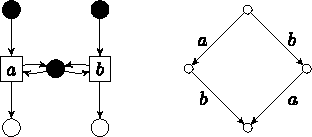
\includegraphics[width=0.95\linewidth,height=0.45\textheight,keepaspectratio]{graphic-01.pdf}\end{center}
 
\begin{center}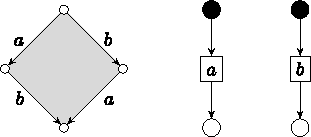
\includegraphics[width=0.95\linewidth,height=0.45\textheight,keepaspectratio]{graphic-02.pdf}\end{center}
  
Figure 1: Petri net and HDA models distinguishing interleaving (left) from non-interleaving (right) concurrency. Left: models for $a.b+b.a$; right: models for $a\parallel b$.\par
 
% END S1.F1
 
% BEGIN S1.p4
 
Muller [37] and Büchi [10] introduced automata recognizing $\omega$-words to study non-terminating sequential machines and decision problems. McNaughton [36] later proved the equivalence of these definitions and extended Kleene’s theorem to $\omega$-words through a non-nested $\omega$-iteration. These automata also have logical [10] and algebraic [11] characterizations. Beyond their theoretical significance, they and their variations (such as Rabin, Streett, and parity automata) play a key role in specifying and verifying reactive systems [14]. This led to the extension of automata models for concurrency to the infinite case, with fundamental results carrying over. For instance, $\omega$-branching automata admit Kleene-like and Büchi-like theorems [31], while similar developments apply to traces [15, 12, 26], leading to decision procedures as corollaries.\par
 
% END S1.p4
 
% BEGIN S1.p5
 
In this paper we introduce higher-dimensional automata for $\omega$-interval pomsets: $\omega$-HDAs. To do so, we first define a class of $\omega$-interval pomsets with interfaces suitable for $\omega$-HDAs and extend the fundamental concepts to the infinite case. This may be effective for modelling (and checking) reactive concurrent systems that may not terminate, especially when reasoning about liveness properties. As in the finite case, we show that isomorphisms of $\omega$-ipomsets are unique and that interval $\omega$-ipomsets admit several equivalent definitions and canonical decompositions. Then we define languages of $\omega$-HDAs in terms of interval $\omega$-ipomsets by considering Büchi and Muller acceptances. We show that unlike HDAs, languages of $\omega$-HDAs may not be closed under subsumption. Thus, we revise the rational operations defined in [19] by ensuring that subsumption is not implicitly assumed and introduce an omega iteration to define $\omega$-rational languages of iipomsets. We show by translating $\omega$-HDAs to $\omega$-automata over discrete ipomsets, called ST-automata, that languages of $\omega$-HDAs are $\omega$-rational. On the other hand, we show that, unlike $\omega$-automata, Büchi acceptance is less expressive than the Muller one in $\omega$-HDAs. In addition, there are $\omega$-rational languages that cannot be recognized by Muller $\omega$-automata. To address this, we initiate first steps towards characterizing the subclass of omega-rational languages that are as expressive as Büchi or Muller $\omega$-HDAs. We refer to the long version [38] for detailed proofs of our results.\par
 
% END S1.p5
 
% END S1


% BEGIN S2
 
\par\medskip\noindent\textbf{2 Ipomsets}\par
 
% BEGIN S2.p1
 
Ipomsets generalize pomsets [29, 40, 28]: a well-established model for non-interleaving concurrency. In this section, we review the fundamental definitions and extend them to the infinite case.\par
 
% END S2.p1
 
% BEGIN S2.SS1
 
\par\medskip\noindent\textbf{2.1 Finite ipomsets}\par
 
% BEGIN S2.SS1.p1
 
We fix a finite alphabet $\Sigma$. An ipomset (over $\Sigma$) is a structure $(P,{<},{\dashrightarrow},S,T,\lambda)$ consisting of a finite set of events $P$, two strict partial orders: $<$ the precedence order, and $\dashrightarrow$ the event order, a set $S\subseteq P$ of source interfaces, a set $T\subseteq P$ of target interfaces such that the elements of $S$ are $<$-minimal and those of $T$ are $<$-maximal, and a labeling function $\lambda:P\to\Sigma$. In addition, we require that the relation ${<}\cup{\dashrightarrow}$ is total, but not necessarily an order. In fact, if we have $x<y$ and $y\dashrightarrow x$, then ${<}\cup{\dashrightarrow}$ is not an order.\par
 
% END S2.SS1.p1
 
% BEGIN S2.SS1.p2
 
For the purpose of notation, we use ${\vphantom{P}}_{S}P_{T}$ for an ipomset $(P,<,\dashrightarrow,S,T,\lambda)$, or refer to it by its set of events $P$ and to its components by adding the subscript P.\par
 
% END S2.SS1.p2
 
% BEGIN S2.SS1.p3
 
We highlight two special cases of ipomsets: conclists $(U,\dashrightarrow,\lambda)$ where $S_{U}=T_{U}=\emptyset$ and $<_{U}=\emptyset$ hence $\dashrightarrow$ total, with $\square$ the set of conclists, and identities $\mathsf{id}_{U}={\vphantom{U}}_{U}U_{U}$ where $S_{U}=T_{U}=U$ and $<_{U}=\emptyset$, with $\mathsf{Id}$ the set of identities. We call $\mathsf{id}_{\emptyset}$ the empty conclist/identity. Note that for any ipomset $P$, $S_{P}=(S,{\dashrightarrow_{\upharpoonleft S\times S}},\lambda_{\upharpoonleft S})$ and $T_{P}=(T,{\dashrightarrow_{\upharpoonleft T\times T}},\lambda_{\upharpoonleft T})$, where “\ensuremath{\upharpoonleft}” denotes restriction, are conclists. An ipomset $P$ is said to be interval (called iipomset) if $<_{P}$ is an interval order, i.e. if for all $w,x,y,z\in P$, if $w<y$ and $x<z$, then $w<z$ or $x<y$.\par
 
% END S2.SS1.p3
 
% BEGIN S2.SS1.p4
 
Let $P$ and $Q$ be two ipomsets. We say that $Q$ subsumes $P$ (written $P\sqsubseteq Q$) if there is a bijection $f:P\to Q$ (a subsumption) such that $\lambda_{Q}\circ f=\lambda_{P}$, $f(S_{P})=S_{Q}$, and $f(T_{P})=T_{Q}$, $\forall x,y\in P,\,f(x)<_{Q}f(y)\Rightarrow x<_{P}y$ and $\forall x,y\in P$ such that $x\nless_{P}y$ and $y\nless_{P}x$, we have $x\dashrightarrow_{P}y\Rightarrow f(x)\dashrightarrow_{Q}f(y)$. Informally speaking, $P$ is more precedence ordered than $Q$.\par
 
% END S2.SS1.p4
 
% BEGIN Thmtheorem1
 
\par\medskip\noindent\textbf{Example 1.}\par
 
% BEGIN Thmtheorem1.p1
 
An example of subsumption is depicted in Fig. 2. Note that $e_{1}<e_{2}$ when the activity interval of $e_{1}$ finishes before the beginning of the one of $e_{2}$. When the activity intervals of two events overlap, they are $\dashrightarrow$-ordered from top to bottom.\par
 
% END Thmtheorem1.p1
 
% END Thmtheorem1
 
% BEGIN S2.SS1.p5
 
An isomorphism of ipomsets is an invertible subsumption (whose inverse is again a subsumption); isomorphic ipomsets are denoted $P\cong Q$. Due to the totality of $<\cup\dashrightarrow$, isomorphisms between ipomsets are unique [4], so we may switch freely between ipomsets and their isomorphism classes. The set of ipomsets is denoted $\mathsf{iPoms}$, and the set of interval ipomsets is written $\mathsf{iiPoms}$.\par
 
% END S2.SS1.p5
 
% BEGIN S2.F2

\begin{center}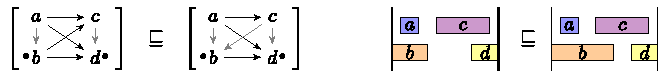
\includegraphics[width=0.95\linewidth,height=0.45\textheight,keepaspectratio]{graphic-03.pdf}\end{center}
 
Figure 2: Ipomsets (left) and their corresponding interval representations (right). Full arrows indicate precedence order; dashed arrows indicate event order; bullets indicate interfaces.\par
 
% END S2.F2
 
% BEGIN S2.SS1.p6
 
In an ipomset $P$, a chain is a subset of $P$ totally ordered by $<_{P}$. An antichain $A$ of $P$ is such that ${<_{P}}\cap(A\times A)=\emptyset$. Hence $A$ is totally ordered by $\dashrightarrow_{P}$. The width of $P$ is ${\mathsf{wd}(P)=\mathsf{sup}{\{|A|\mathrel{\big{|}}A\text{ is an $<$-antichain of }P\}}}$.\par
 
% END S2.SS1.p6
 
% END S2.SS1
 
% BEGIN S2.SS2
 
\par\medskip\noindent\textbf{2.2 The set of $\omega$-ipomsets}\par
 
% BEGIN S2.SS2.p1
 
Similarly to ipomsets, an $\omega$-ipomset is a structure of the form $(P,{<},{\dashrightarrow},S,\lambda)$. The only changes are that $P$ is countably infinite and there is no target interface. However, let $\Omega_{P}$ denote the set of all $<_{P}$-maximal elements. This is not similar to a target interface: even if $\Omega_{P}$ represents unfinished events, terminating them (by trying to glue an ipomset after $P$) may cause chains greater than $\omega$.\par
 
% END S2.SS2.p1
 
% BEGIN S2.SS2.p2
 
For the remainder of the paper, we focus on a subclass of $\omega$-ipomsets.\par
 
% END S2.SS2.p2
 
% BEGIN Thmtheorem2
 
\par\medskip\noindent\textbf{Definition 2 (Valid $\omega$-ipomset).}\par
 
% BEGIN Thmtheorem2.p1
 
A valid $\omega$-ipomset is an $\omega$-ipomset $P$ such that\par
  
\par\noindent  $\blacksquare$ 
% BEGIN S2.I1.i1.p1
 
$\forall x\in P,\,{\{y\mathrel{\big{|}}y<_{P}x\}}$ is finite;\par
 
% END S2.I1.i1.p1
 
 
\par\noindent  $\blacksquare$ 
% BEGIN S2.I1.i2.p1
 
every $<_{P}$-antichain of $P$ is finite.\par
 
% END S2.I1.i2.p1
 
  
% END Thmtheorem2.p1
 
% END Thmtheorem2
 
% BEGIN S2.SS2.p3
 
The first point is here to forbid $\omega$-ipomsets with chains greater than $\omega$, and therefore extend properly classical $\omega$-words and $\omega$-pomsets [31]. It is a classical property required in event structures (see [44] for example). The second point is to avoid an infinite number of concurrent events. This condition implies in particular that $S_{P}$ and $\Omega_{P}$ are finite. Both conditions also imply that $<_{P}$ is a well quasi-order, but the converse is not true. In the rest of this paper, unless specified, we will talk about valid $\omega$-ipomsets, and will omit the word “valid”.\par
 
% END S2.SS2.p3
 
% BEGIN S2.SS2.p4
 
Let $P$ and $Q$ be two (valid) $\omega$-ipomsets. We define the subsumption $P\sqsubseteq Q$ as in the finite case by preserving also the $<_{P}$-maximal elements $\Omega_{P}$. Again, isomorphisms of $\omega$-ipomsets are invertible subsumptions (whose inverse is again a subsumption). The first result of this paper is the unicity of these isomorphisms. The proof is similar to the finite case, using pomset filtration (see [18, Lem. 34]):\par
 
% END S2.SS2.p4
 
% BEGIN Thmtheorem3
 
\par\medskip\noindent\textbf{Proposition 3.}\par
 
% BEGIN Thmtheorem3.p1
 
Isomorphisms between $\omega$-ipomsets are unique.\par
 
% END Thmtheorem3.p1
 
% END Thmtheorem3
 
% BEGIN S2.SS2.p5
 
Note that the proposition does not hold for general (non-valid) $\omega$-ipomsets: for example, all shifts by $n\in\mathbb{Z}$ are non-trivial automorphisms of $\mathbb{Z}$. As in the finite case, we may now switch freely between $\omega$-ipomsets and their isomorphism classes. The set of $\omega$-ipomsets is denoted ${\mathsf{iPoms}^{\omega}}$, and we use the notation ${\mathsf{iPoms}^{\infty}}\coloneqq\mathsf{iPoms}\cup{\mathsf{iPoms}^{\omega}}$.\par
 
% END S2.SS2.p5
 
% END S2.SS2
 
% BEGIN S2.SS3
 
\par\medskip\noindent\textbf{2.3 Operations on $\omega$-ipomsets}\par
 
% BEGIN S2.SS3.p1
 
We extend here the operations $*$ (gluing) and $\parallel$ (parallel composition) to $\omega$-ipomsets.\par
 
% END S2.SS3.p1
 
% BEGIN S2.SS3.p2
 
For $(P,Q)\in({\mathsf{iPoms}^{\infty}}\times{\mathsf{iPoms}^{\infty}})\setminus(\mathsf{iPoms}\times\mathsf{iPoms})$, the parallel composition $P\parallel Q$ (or $\left[\begin{smallmatrix}P\\
Q\end{smallmatrix}\right]$) is the $\omega$-ipomset $(P\sqcup Q,\,<_{P}\sqcup<_{Q},\,\dashrightarrow,\,S_{P}\sqcup S_{Q},\,\lambda_{P}\sqcup\lambda_{Q})$ where $\sqcup$ is the disjoint union and $x\dashrightarrow y$ iff $(x,y)\in P\times Q$ or $x\dashrightarrow_{P}y$ or $x\dashrightarrow_{Q}y$.\par
 
% END S2.SS3.p2
 
% BEGIN S2.SS3.p3
 
The gluing composition $P*Q$ (or $PQ$ ) of $(P,Q)\in\mathsf{iPoms}\times{\mathsf{iPoms}^{\omega}}$ is defined if there exists a unique111Isomorphisms of conclists is a special case of ipomset isomorphisms. Unicity is ensured by event order. isomorphism $f\colon T_{P}\to S_{Q}$, by $((P\sqcup Q)_{/x\sim f(x)},<,\dashrightarrow,S_{P},\lambda_{P}\cup\lambda_{Q})$222($P\sqcup Q)_{x\sim f(x)}$ is the quotient of the disjoint union under the unique isomorphism $f:T_{P}\to S_{Q}$., where:\par
  
\par\noindent  $\blacksquare$ 
% BEGIN S2.I2.i1.p1
 
$x<y$ iff $x<_{P}y$, $x<_{Q}y$, or $x\in P\setminus T_{P}$ and $y\in Q\setminus S_{Q}$;\par
 
% END S2.I2.i1.p1
 
 
\par\noindent  $\blacksquare$ 
% BEGIN S2.I2.i2.p1
 
$\dashrightarrow$ is the transitive closure of $\dashrightarrow_{P}\cup\dashrightarrow_{Q}$ on $(P\sqcup Q)_{/x\sim f(x)}$.\par
 
% END S2.I2.i2.p1
 
  
Informally, the sources of $Q$ are attached to the targets of $P$.\par
 
% END S2.SS3.p3
 
% BEGIN S2.SS3.p4
 
Note that both $*$ and $\parallel$ are associative and non-commutative. The non-commutativity of $\parallel$ is due to event order. The latter is crucial for isomorphism unicity and to define gluing composition. Still, even if $\left[\begin{smallmatrix}a\\
b\end{smallmatrix}\right]\neq\left[\begin{smallmatrix}b\\
a\end{smallmatrix}\right]$, both express that $a$ and $b$ are running concurrently. Alur et al in [1] introduced a similar “ordered parallel composition” for application purposes.\par
 
% END S2.SS3.p4
 
% BEGIN S2.SS3.p5
 
We also introduce an infinite gluing of an $\omega$-sequence of ipomsets. Let $(P_{i})_{i\in\mathbb{N}}\in\mathsf{iPoms}^{\mathbb{N}}$ such that for all $i$, $T_{P_{i}}\cong S_{P_{i\text{+}1}}$. We define $P=P_{0}*P_{1}*\cdots$ by $(P,<,\dashrightarrow,S_{P},\lambda_{P})$, where\par
  
\par\noindent  $\blacksquare$ 
% BEGIN S2.I3.i1.p1
 
$P=(\bigcup\nolimits_{i\in\mathbb{N}}(P_{i},i))_{/x\sim f(x)}$ where $f:\bigcup\nolimits_{i\in\mathbb{N}}(T_{i},i)\rightarrow\bigcup\nolimits_{i\in\mathbb{N}}(S_{i},i)$ such that $f(x,i)=(f_{i}(x),$ $i+1)$ with $f_{i}$ the unique isomorphism between $T_{P_{i}}$ and $S_{P_{i\text{+}1}}$;\par
 
% END S2.I3.i1.p1
 
 
\par\noindent  $\blacksquare$ 
% BEGIN S2.I3.i2.p1
 
$S_{P}=S_{P_{0}}\times{\{0\}}$;\par
 
% END S2.I3.i2.p1
 
 
\par\noindent  $\blacksquare$ 
% BEGIN S2.I3.i3.p1
 
$(x,i)<_{P}(y,j)$ if ($i=j$ and $x<_{P_{i}}y$) or ($i\text{+}1\leqslant j$, $x\in P_{i}\setminus T_{P_{i}}$ and $y\in P_{i\text{+}1}\setminus S_{P_{i\text{+}1}}$);\par
 
% END S2.I3.i3.p1
 
 
\par\noindent  $\blacksquare$ 
% BEGIN S2.I3.i4.p1
 
$\dashrightarrow_{P}$ is the transitive closure of $\bigcup_{i\in\mathbb{N}}\dashrightarrow_{P_{i}}$;\par
 
% END S2.I3.i4.p1
 
 
\par\noindent  $\blacksquare$ 
% BEGIN S2.I3.i5.p1
 
$\lambda_{P}(x,i)=\lambda_{P_{i}}(x)$ for $i\in\mathbb{N}$ and $x\in P_{i}$.\par
 
% END S2.I3.i5.p1
 
  
% END S2.SS3.p5
 
% BEGIN S2.SS3.p6
 
Note in particular that when $P_{i}\in\mathsf{Id}$ we have $P_{0}*\dots*P_{i-1}*P_{i}*P_{i+1}*\dots=P_{0}*\dots*P_{i-1}*P_{i+1}*\cdots$. We let denote by $P^{\omega}$ the $\omega$-ipomset defined by the infinite gluing of the constant sequence equal to $P$ with $S_{P}\cong T_{P}$.\par
 
% END S2.SS3.p6
 
% BEGIN Thmtheorem4
 
\par\medskip\noindent\textbf{Lemma 4.}\par
 
% BEGIN Thmtheorem4.p1
 
For $(P_{i})_{i\in\mathbb{N}}\in\mathsf{iPoms}^{\mathbb{N}}$ with $T_{P_{i}}\cong S_{P_{i\text{+}1}}$, $P=P_{0}*P_{1}*\cdots$ is valid if the number of $P_{i}\in\mathsf{iPoms}\setminus\mathsf{Id}$ is infinite and there exists $m\in\mathbb{N}$ such that for all $i\in\mathbb{N},\leavevmode\nobreak\ \mathsf{wd}(P_{i})\leqslant m$.\par
 
% END Thmtheorem4.p1
 
% END Thmtheorem4
 
% BEGIN S2.SS3.p7
 
Intuitively, $P$ is infinite since it is obtained by composing infinitely many non-identities, finite past is a consequence of the infinite gluing definition, and finiteness of antichains is due to width-boundedness of the operands. Note that this is not an equivalence condition. The infinite gluing may define a valid $\omega$-ipomset even if $\mathsf{wd}(P_{i})$ are not bounded (see Fig. 3). Finding an equivalence condition on $(P_{i})$ is hard, because it has to consider event order. For example, Fig. 6 exhibits two infinite products behaving differently with only a change of event order.\par
 
% END S2.SS3.p7
 
% BEGIN S2.F3

\begin{center}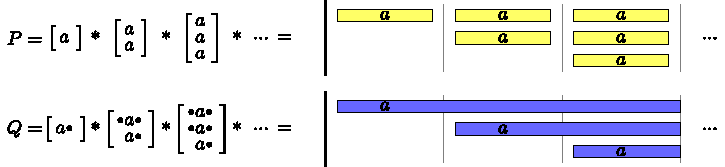
\includegraphics[width=0.95\linewidth,height=0.45\textheight,keepaspectratio]{graphic-04.pdf}\end{center}
 
Figure 3: Two unbounded infinite products giving a valid (up) and an invalid (down) $\omega$-ipomset.\par
 
% END S2.F3
 
% END S2.SS3
 
% BEGIN S2.SS4
 
\par\medskip\noindent\textbf{2.4 Interval $\omega$-ipomsets}\par
 
% BEGIN S2.SS4.p1
 
We will here only deal with interval $\omega$-ipomsets. An $\omega$-ipomset is interval (denoted $\omega$-iipomset) if for all $w,x,y,z\in P$, if $w<y$ and $x<z$, then $w<z$ or $x<y$. The set of all interval $\omega$-ipomsets is denoted ${\mathsf{iiPoms}^{\omega}}$ (and we use the notation ${\mathsf{iiPoms}^{\infty}}\coloneqq\mathsf{iiPoms}\cup{\mathsf{iiPoms}^{\omega}}$).\par
 
% END S2.SS4.p1
 
% BEGIN S2.SS4.p2
 
There are multiple equivalent ways to define interval ipomsets [18, Lem. 39], and the same goes for $\omega$-ipomsets.\par
 
% END S2.SS4.p2
 
% BEGIN S2.SS4.p3
 
We say that $P\in{\mathsf{iPoms}^{\omega}}$ admits an interval representation if there are two functions ${b,e:P\rightarrow\mathbb{N}\cup{\{+\infty\}}}$ such that for all $x,y\in P$, $b(x)\leqslant e(x)$ and $x<_{P}y\Leftrightarrow e(x)<b(y)$.\par
 
% END S2.SS4.p3
 
% BEGIN S2.SS4.p4
 
As for finite pomsets and with similar arguments, the following holds:\par
 
% END S2.SS4.p4
 
% BEGIN Thmtheorem5
 
\par\medskip\noindent\textbf{Proposition 5.}\par
 
% BEGIN Thmtheorem5.p1
 
Let $P$ be an $\omega$-ipomset, the following are equivalent:\par
  
\par\noindent  1. 
% BEGIN S2.I4.i1.p1
 
$P$ is an interval $\omega$-ipomset;\par
 
% END S2.I4.i1.p1
 
 
\par\noindent  2. 
% BEGIN S2.I4.i2.p1
 
$P$ has an interval representation;\par
 
% END S2.I4.i2.p1
 
 
\par\noindent  3. 
% BEGIN S2.I4.i3.p1
 
the order $\ll$ on maximal antichains of $P$ defined by $A\ll B$ iff $A\neq B$ and $\forall(a,b)\in A\times B$, $b\nless_{P}a$ is linear.\par
 
% END S2.I4.i3.p1
 
  
% END Thmtheorem5.p1
 
% END Thmtheorem5
 
% BEGIN S2.SS4.p5
 
Establishing the equivalence between the first two items is a routine. The third item is less intuitive, but it implies the second one by showing that the set of maximal antichains equipped with $\ll$ is isomorphic to $(\mathbb{N},<)$. From that, to an event $a\in P$ we can associate the interval going from the index of the first appearance of $a$ in the antichains to the index of the last appearance.\par
 
% END S2.SS4.p5
 
% BEGIN Thmtheorem6
 
\par\medskip\noindent\textbf{Example 6.}\par
 
% BEGIN Thmtheorem6.p1
 
The minimal non-interval ipomset $aa\parallel bb$ can be generalized to the non-interval $\omega$-ipomset $a^{\omega}\parallel b^{\omega}$, while $(a\parallel b)^{\omega}\in{\mathsf{iiPoms}^{\omega}}$, as well as $\left[\begin{smallmatrix}\vbox{\hbox{\tiny$\bullet$}}aa\vbox{\hbox{\tiny$\bullet$}}\\
b\end{smallmatrix}\right]^{\omega}$ represented in Fig. 4.\par
 
% END Thmtheorem6.p1
 
% END Thmtheorem6
 
% BEGIN S2.F4
  
\begin{center}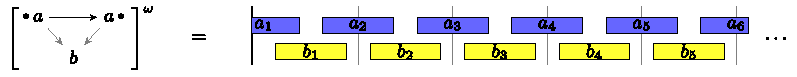
\includegraphics[width=0.95\linewidth,height=0.45\textheight,keepaspectratio]{graphic-05.pdf}\end{center}
   
\begin{center}\resizebox{\linewidth}{!}{$\begin{aligned}\displaystyle{\{a_{1},b_{1}\}}\ll{\{b_{1},a_{2}\}}\ll{\{a_{2},b_{2}\}} & \displaystyle\ll{\{b_{2},a_{3}\}}\ll{\{a_{3},b_{3}\}}\ll{\{b_{3},a_{4}\}}\ll{\{a_{4},b_{4}\}}\ll...\end{aligned}$}\end{center}
   
Figure 4: Interval representation and linear order on antichains of the $\omega$-iipomset of Ex. 6.\par
 
% END S2.F4
 
% END S2.SS4
 
% BEGIN S2.SS5
 
\par\medskip\noindent\textbf{2.5 Decomposition of $\omega$-iipomsets}\par
 
% BEGIN S2.SS5.p1
 
A starter $U$ is a discrete ipomset (i.e. $<_{U}$ is empty) with $T_{U}=U$ (hence written ${\vphantom{U}}_{S}U_{U}$), and a terminator $U$ is a discrete ipomset with $S_{U}=U$ (written ${\vphantom{U}}_{U}U_{T}$). We denote by $\Xi$ the set of starters and terminators. Note that $\mathsf{Id}\subseteq\Xi$. We say that $U\in\Xi$ is proper if $U\in\Xi\setminus\mathsf{Id}$. A starter ${\vphantom{U}}_{U-A}U_{U}$ will be written ${}_{A\!}{\uparrow}{U}$ (meaning it contains the events in $U$ and start the events in $A\subseteq U$), and a terminator ${\vphantom{U}}_{U}U_{U-A}$ will be written ${U}{\downarrow}_{A}$. We call a step decomposition of $P\in{\mathsf{iPoms}^{\omega}}$ a sequence of starters and terminators $(U_{i})_{i\in\mathbb{N}}$ such that $P=U_{0}*U_{1}*\cdots$, and a decomposition is said to be sparse if proper starters and terminators are alternating. As for finite iipomsets [22], we can prove uniqueness of sparse decompositions of $\omega$-iipomsets:\par
 
% END S2.SS5.p1
 
% BEGIN Thmtheorem7
 
\par\medskip\noindent\textbf{Theorem 7.}\par
 
% BEGIN Thmtheorem7.p1
 
Every interval $\omega$-ipomset has a unique sparse step decomposition.\par
 
% END Thmtheorem7.p1
 
% END Thmtheorem7
 
% BEGIN S2.F5

\begin{center}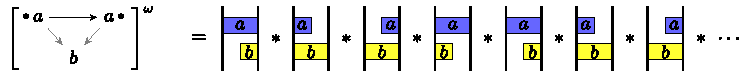
\includegraphics[width=0.95\linewidth,height=0.45\textheight,keepaspectratio]{graphic-06.pdf}\end{center}
 
Figure 5: Sparse decomposition of Ex. 6.\par
 
% END S2.F5
 
% BEGIN Thmtheorem8
 
\par\medskip\noindent\textbf{$\blacktriangleright$ Remark 8.}\par
 
% BEGIN Thmtheorem8.p1
 
In Th. 7, $\omega$-ipomsets are in ${\mathsf{iiPoms}^{\omega}}$ so supposed valid, thus we do not have to verify that the infinite product effectively gives a valid result. Indeed, an infinite product of alternating proper starters and terminators may yield a non-valid $\omega$-ipomset (see Fig. 6).\par
 
% END Thmtheorem8.p1
 
% END Thmtheorem8
 
% BEGIN S2.F6

\begin{center}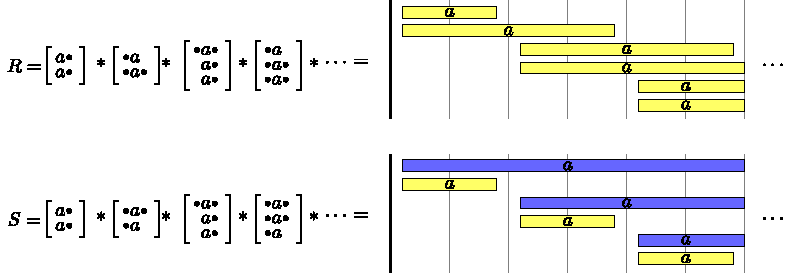
\includegraphics[width=0.95\linewidth,height=0.45\textheight,keepaspectratio]{graphic-07.pdf}\end{center}
 
Figure 6: Two sparse decompositions with different event orders, such that only $R$ is valid.\par
 
% END S2.F6
 
% BEGIN S2.SS5.p2
 
Defining such a decomposition gives us a characterization of $\omega$-iipomsets in terms of their prefixes. We say that $A\in\mathsf{iPoms}$ is a (finite) prefix of $P\in{\mathsf{iPoms}^{\infty}}$ if there is $Q\in{\mathsf{iPoms}^{\infty}}$ such that $P=AQ$, and then write $A\prec P$. We call $\mathsf{Pref}(P)$ the set of all prefixes of $P$.\par
 
% END S2.SS5.p2
 
% BEGIN Thmtheorem9
 
\par\medskip\noindent\textbf{$\blacktriangleright$ Remark 9.}\par
 
% BEGIN Thmtheorem9.p1
 
Unlike classical $\omega$-words theory, two prefixes of $P$ may be incomparable, for example $a\vbox{\hbox{\tiny$\bullet$}}\prec\left[\begin{smallmatrix}a\\
b\end{smallmatrix}\right]$ and $b\vbox{\hbox{\tiny$\bullet$}}\prec\left[\begin{smallmatrix}a\\
b\end{smallmatrix}\right]$ but $a\vbox{\hbox{\tiny$\bullet$}}\not\prec b\vbox{\hbox{\tiny$\bullet$}}$ and $b\vbox{\hbox{\tiny$\bullet$}}\not\prec a\vbox{\hbox{\tiny$\bullet$}}$. But we still have the property that for $A\in\mathsf{Pref}(P)$ and $x\in A$, if $y<_{P}x$ then $y\in A$. Note that neither $a\vbox{\hbox{\tiny$\bullet$}}$ nor $b\vbox{\hbox{\tiny$\bullet$}}$ could be the first step of the sparse decomposition of $(a\parallel b)^{\omega}$. Its only possible first step is $\left[\begin{smallmatrix}a\vbox{\hbox{\tiny$\bullet$}}\\
b\vbox{\hbox{\tiny$\bullet$}}\end{smallmatrix}\right]$.\par
 
% END Thmtheorem9.p1
 
% END Thmtheorem9
 
% BEGIN S2.SS5.p3
 
The following lemma is trivial in classical $\omega$-word theory, but here relies crucially on the fact that we deal with valid $\omega$-ipomsets.\par
 
% END S2.SS5.p3
 
% BEGIN Thmtheorem10
 
\par\medskip\noindent\textbf{Lemma 10.}\par
 
% BEGIN Thmtheorem10.p1
 
If $(A_{i})_{i\in I}$ is an infinite set of prefixes of an $\omega$-ipomset $P$, and $R$ is a finite subset of $P$ (seen as a set), then there is $i\in I$ such that $R\subseteq A_{i}$.\par
 
% END Thmtheorem10.p1
 
% END Thmtheorem10
 
% BEGIN S2.SS5.SSS0.P0.SPx1
 
\par\medskip\noindent\textbf{Proof.}\par
 
% BEGIN S2.SS5.SSS0.P0.SPx1.p1
 
Let $(A_{i})_{i\in I}\in\mathsf{Pref}(P)^{I}$ (with $I$ infinite), and $x\in R$. We want to prove that the set ${\{A_{i}\mathrel{\big{|}}x\in A_{i}\}}$ is infinite. Let $x\in P$, and $P^{m}$ be (the antichain of) the $<$-minimal elements of ${\{x\}}\cup{\{p\in P\mathrel{\big{|}}x\not<p\text{ and }p\not<x\}}$, and $Q:=P^{m}\cup{\{p\in P\mathrel{\big{|}}p<x\}}$. As $P$ is valid, $Q$ is finite, and so there is a finite number of ipomsets included in $Q$. Thus there is an infinite number of $A_{i}\text{ s.t.\ }A_{i}\cap(P-Q)\neq\emptyset$. In such $A_{i}$, let $y_{i}\in A_{i}\cap(P-Q)$. There is an element $z_{i}\in P^{m}\text{ s.t.\ }z_{i}<y_{i}$: either $x<y_{i}$ (and so $z_{i}=x$), or $y_{i}\in{\{p\in P\mathrel{\big{|}}x\not<p\text{ and }p\not<x\}}$ (and so there is $z_{i}\in P^{m}\subseteq Q$ such that $z_{i}\leqslant y_{i}$, and $z_{i}\neq y_{i}$ as $z_{i}\in Q$ and $y_{i}\not\in Q$). As $A_{i}$ is a prefix of $P$, $y_{i}\in A_{i}$ implies that $z_{i}$ is necessarily in $A_{i}-T_{A_{i}}$, and so $x\in A_{i}$ (otherwise $x\in B_{i}-S_{B_{i}}$ with $P=A_{i}*B_{i}$ and so $z_{i}<x$, which is impossible because $P^{m}$ is an antichain). So there are infinitely many $A_{i}$ such that $x\in A_{i}$.\par
 
% END S2.SS5.SSS0.P0.SPx1.p1
 
% BEGIN S2.SS5.SSS0.P0.SPx1.p2
 
Then, we take $(A_{i})_{i\in I^{\prime}}$, an infinite set of prefixes of $P$ that all contain $x$, and we iteratively use the previous argument to get all elements of the (finite) set $R$. At the end we have $(A_{i})_{i\in J}$, an infinite set of prefixes of $P$ that all contain $R$, and we conclude the proof by taking anyone of them. $\hfill\blacktriangleleft$\par
 
% END S2.SS5.SSS0.P0.SPx1.p2
 
% BEGIN Thmtheorem11
 
\par\medskip\noindent\textbf{$\blacktriangleright$ Remark 11.}\par
 
% BEGIN Thmtheorem11.p1
 
Note that $P$ is not necessarily interval in Lem. 10. It only suffices to have an infinite number of prefixes. However being an interval $\omega$-ipomset ensures the existence of an infinite set of prefixes, see below. For example, $P=a^{\omega}\parallel b^{\omega}\not\in{\mathsf{iiPoms}^{\omega}}$ has a finite number of prefixes: $\mathsf{Pref}(P)={\{a\vbox{\hbox{\tiny$\bullet$}},b\vbox{\hbox{\tiny$\bullet$}},\left[\begin{smallmatrix}a\vbox{\hbox{\tiny$\bullet$}}\\
b\vbox{\hbox{\tiny$\bullet$}}\end{smallmatrix}\right]\}}$, while $Q=(aa\parallel bb).c^{\omega}\not\in{\mathsf{iiPoms}^{\omega}}$ has an infinite number of prefixes: $\mathsf{Pref}(Q)\supseteq{\{(aa\parallel bb).c^{n}\mathrel{\big{|}}n\in\mathbb{N}\}}$.\par
 
% END Thmtheorem11.p1
 
% END Thmtheorem11
 
% BEGIN S2.SS5.SSS0.P0.SPx1.p3
 
From Lem. 10 follows a sequential characterization of interval $\omega$-ipomsets:\par
 
% END S2.SS5.SSS0.P0.SPx1.p3
 
% BEGIN Thmtheorem12
 
\par\medskip\noindent\textbf{Proposition 12.}\par
 
% BEGIN Thmtheorem12.p1
 
Let $P$ be an $\omega$-ipomset, the following are equivalent:\par
  
\par\noindent  1. 
% BEGIN S2.I5.i1.p1
 
$P$ is an interval $\omega$-ipomset;\par
 
% END S2.I5.i1.p1
 
 
\par\noindent  2. 
% BEGIN S2.I5.i2.p1
 
$\mathsf{Pref}(P)$ is infinite and for all $A\in\mathsf{Pref}(P)$, $A$ is an interval ipomset;\par
 
% END S2.I5.i2.p1
 
 
\par\noindent  3. 
% BEGIN S2.I5.i3.p1
 
an infinite number of prefixes of $P$ are interval ipomsets.\par
 
% END S2.I5.i3.p1
 
  
% END Thmtheorem12.p1
 
% END Thmtheorem12
 
% BEGIN S2.SS5.SSS0.P0.SPx1.p4
 
In addition, from the last point of Prop. 12 along with the preservation of the interval property by gluing composition (see [18, Lem. 41]) we have the following:\par
 
% END S2.SS5.SSS0.P0.SPx1.p4
 
% BEGIN Thmtheorem13
 
\par\medskip\noindent\textbf{Corollary 13.}\par
 
% BEGIN Thmtheorem13.p1
 
If $P=P_{0}*P_{1}*\cdots$ is a valid $\omega$-ipomset and $\forall i\in\mathbb{N},\,P_{i}\in\mathsf{iiPoms}$, then $P\in{\mathsf{iiPoms}^{\omega}}$.\par
 
% END Thmtheorem13.p1
 
% END Thmtheorem13
 
% END S2.SS5.SSS0.P0.SPx1
 
% END S2.SS5
 
% END S2


% BEGIN S3
 
\par\medskip\noindent\textbf{3 Higher-dimensional automata}\par
 
% BEGIN S3.p1
 
In this section, we recall higher-dimensional automata (HDAs) over iipomsets [7, 18, 22] and introduce $\omega$-HDAs. Recall that $\square$ denotes the set of conclists.\par
 
% END S3.p1
 
% BEGIN S3.SS1
 
\par\medskip\noindent\textbf{3.1 HDAs over finite ipomsets}\par
 
% BEGIN S3.SS1.p1
 
A precubical set is a structure $(X,\mathsf{ev},\Delta)$ with:\par
  
\par\noindent  $\blacksquare$ 
% BEGIN S3.I1.i1.p1
 
a set of cells $X$;\par
 
% END S3.I1.i1.p1
 
 
\par\noindent  $\blacksquare$ 
% BEGIN S3.I1.i2.p1
 
a function $\mathsf{ev}:X\rightarrow\square$ which assigns to a cell its list of active events (for $U\in\square$ we write $X[U]={\{q\in X\mathrel{\big{|}}\mathsf{ev}(x)=U\}}$);\par
 
% END S3.I1.i2.p1
 
 
\par\noindent  $\blacksquare$ 
% BEGIN S3.I1.i3.p1
 
face maps $\Delta={\{\delta_{A,U}^{0},\,\delta_{A,U}^{1}\mathrel{\big{|}}U\in\square,\,A\subseteq U\}}$ such that $\delta_{A,U}^{0},\delta_{A,U}^{1}:X[U]\rightarrow X[U-A]$;\par
 
% END S3.I1.i3.p1
 
 
\par\noindent  $\blacksquare$ 
% BEGIN S3.I1.i4.p1
 
for $A,B\subseteq U\text{ s.t.\ }A\cap B=\emptyset$ and $\mu,\nu\in{\{0,1\}}$, we have the following precubical identities: $\delta_{A,U-B}^{\mu}\circ\delta_{B,U}^{\nu}=\delta_{B,U-A}^{\nu}\circ\delta_{A,U}^{\mu}$.\par
 
% END S3.I1.i4.p1
 
  
We usually refer to a precubical set by its set of cells $X$, and for face maps we often omit the second subscript $U$. The dimension of a cell $q\in X$ is the size $|\mathsf{ev}(q)|$. An upper face map $\delta_{A}^{1}$ terminates the events in $A$, whereas a lower face map $\delta_{A}^{0}$ “unstarts” these events, that is, it maps to a cell where the events of $A$ are not yet started.\par
 
% END S3.SS1.p1
 
% BEGIN S3.SS1.p2
 
A higher-dimensional automaton is a tuple $(X,\bot_{X},\top_{X})$ where $X$ is a finite precubical set, and $\bot_{X},\top_{X}\subseteq X$ are the sets of starting and accepting cells. We may omit the subscripts X if the context is clear, and refer to an HDA only by its precubical set.\par
 
% END S3.SS1.p2
 
% BEGIN Thmtheorem14
 
\par\medskip\noindent\textbf{Example 14.}\par
 
% BEGIN Thmtheorem14.p1
 
Fig. 7 shows a two-dimensional HDA as a combinatorial object (left) and in a geometric realisation (right). The arrows between the cells on the left representation correspond to the face maps connecting them. It consists of nine cells: the corner cells $X_{0}=\{x,y,v,w\}$ in which no event is active (for all $z\in X_{0}$, $\mathsf{ev}(z)=\emptyset$), the transition cells $X_{1}=\{g,h,f,e\}$ in which one event is active ($\mathsf{ev}(f)=\mathsf{ev}(e)=a$ and $\mathsf{ev}(g)=\mathsf{ev}(h)=b$), and the square cell $q$ where $\mathsf{ev}(q)=\left[\begin{smallmatrix}a\\
b\end{smallmatrix}\right]$. By convention, for $a\dashrightarrow b$, we represent the event $a$ horizontally and the event $b$ vertically.\par
 
% END Thmtheorem14.p1
 
% END Thmtheorem14
 
% BEGIN S3.F7

\begin{center}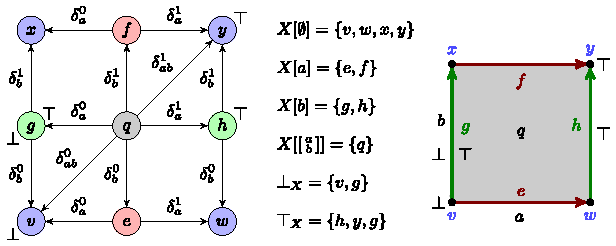
\includegraphics[width=0.95\linewidth,height=0.45\textheight,keepaspectratio]{graphic-08.pdf}\end{center}
 
Figure 7: A two-dimensional HDA $X$ on $\Sigma=\{a,b\}$, see Ex. 14.\par
 
% END S3.F7
 
% BEGIN S3.SS1.p3
 
A track $\alpha$ in $X$ is a sequence $(q_{0},\varphi_{1},q_{1},\dots,\varphi_{n},q_{n})$ where $q_{i}\in X$ are cells and $\varphi_{i}$ denote face map types. That is, for all $i\leqslant n$, $(q_{i},\varphi_{i},q_{i\text{+}1})$ is:\par
  
\par\noindent  $\blacksquare$ 
% BEGIN S3.I2.i1.p1
 
either an upstep: $(\delta_{A}^{0}(q_{i\text{+}1}),\mathrel{\nearrow^{A}},q_{i\text{+}1})$ with $A\subseteq\mathsf{ev}(q_{i\text{+}1})$,\par
 
% END S3.I2.i1.p1
 
 
\par\noindent  $\blacksquare$ 
% BEGIN S3.I2.i2.p1
 
or a downstep: $(q_{i},\mathrel{\searrow_{B}},\delta_{B}^{1}(q_{i}))$ with $B\subseteq\mathsf{ev}(q_{i})$.\par
 
% END S3.I2.i2.p1
 
  
The source of $\alpha$ is $\mathsf{src}(\alpha)=q_{0}$ and its target is $\mathsf{tgt}(\alpha)=q_{n}$. A track is accepting if $\mathsf{src}(\alpha)\in\bot_{X}$ and $\mathsf{tgt}(\alpha)\in\top_{X}$. Note that tracks are concatenations (denoted using $*$) of upsteps and downsteps. The language of an HDA is defined in terms of the event ipomsets of its accepting tracks. Formally, the event ipomset of a track $\alpha$ (written $\mathsf{ev}(\alpha)$) is defined by:\par
  
\par\noindent  $\blacksquare$ 
% BEGIN S3.I3.i1.p1
 
$\mathsf{ev}((q))=\mathsf{id}_{\mathsf{ev}(q)}$ (with $q\in X$ and $(q)$ a single-cell track)\par
 
% END S3.I3.i1.p1
 
 
\par\noindent  $\blacksquare$ 
% BEGIN S3.I3.i2.p1
 
$\mathsf{ev}((q,\mathrel{\nearrow^{A}},p))={}_{A\!}{\uparrow}{\mathsf{ev}(p)}$ (the starter which starts events $A$)\par
 
% END S3.I3.i2.p1
 
 
\par\noindent  $\blacksquare$ 
% BEGIN S3.I3.i3.p1
 
$\mathsf{ev}((q,\mathrel{\searrow_{B}},p))={\mathsf{ev}(q)}{\downarrow}_{B}$ (the terminator which terminates events $B$)\par
 
% END S3.I3.i3.p1
 
 
\par\noindent  $\blacksquare$ 
% BEGIN S3.I3.i4.p1
 
$\mathsf{ev}(\alpha_{1}*\dots*\alpha_{n})=\mathsf{ev}(\alpha_{1})*\dots*\mathsf{ev}(\alpha_{n})$\par
 
% END S3.I3.i4.p1
 
  
We say that two tracks $\alpha$ and $\beta$ are equivalent, denoted $\alpha\simeq\beta$, with $\simeq$ the relation generated by the three cases $(x\mathrel{\nearrow^{A}}y\mathrel{\nearrow^{B}}z)\simeq(x\mathrel{\nearrow^{A\cup B}}z)$, $(x\mathrel{\searrow_{A}}y\mathrel{\searrow_{B}}z)\simeq(x\mathrel{\searrow_{A\cup B}}z)$, and $\gamma\alpha\delta\simeq\gamma\beta\delta$ whenever $\alpha\simeq\beta$. Basically, two tracks are equivalent if their “contractions” into sparse tracks (i.e. alternating upsteps and downsteps) and event ipomsets are equal.\par
 
% END S3.SS1.p3
 
% BEGIN Thmtheorem15
 
\par\medskip\noindent\textbf{Example 15.}\par
 
% BEGIN Thmtheorem15.p1
 
The HDA $X$ of Fig. 7 admits several accepting tracks with target $h$, for example $v\mathrel{\nearrow^{ab}}q\mathrel{\searrow_{a}}h$. This is a sparse track and equivalent to the non-sparse tracks $v\mathrel{\nearrow^{a}}e\mathrel{\nearrow^{b}}q\mathrel{\searrow_{a}}h$ and $v\mathrel{\nearrow^{b}}g\mathrel{\nearrow^{a}}q\mathrel{\searrow_{a}}h$. Their event ipomset is $\left[\begin{smallmatrix}a\hphantom{\vbox{\hbox{\tiny$\bullet$}}}\\
b\vbox{\hbox{\tiny$\bullet$}}\end{smallmatrix}\right]$. The track $v\mathrel{\nearrow^{a}}e\mathrel{\searrow_{a}}w\mathrel{\nearrow^{b}}h$ is also accepting with event ipomset $ab\vbox{\hbox{\tiny$\bullet$}}\sqsubseteq\left[\begin{smallmatrix}a\hphantom{\vbox{\hbox{\tiny$\bullet$}}}\\
b\vbox{\hbox{\tiny$\bullet$}}\end{smallmatrix}\right]$. In addition, since $g$ is both a start and accept cell, we have also $g$ and $v\mathrel{\nearrow^{b}}g$ as accepting tracks, with event ipomsets $\vbox{\hbox{\tiny$\bullet$}}b\vbox{\hbox{\tiny$\bullet$}}$ and $b\vbox{\hbox{\tiny$\bullet$}}$, respectively. Note that tracks move forward along upper face maps but backward along lower ones. $X$ accept tracks whose ipomsets are in ${\{b\vbox{\hbox{\tiny$\bullet$}},\vbox{\hbox{\tiny$\bullet$}}b\vbox{\hbox{\tiny$\bullet$}},ab\vbox{\hbox{\tiny$\bullet$}},\left[\begin{smallmatrix}a\hphantom{\vbox{\hbox{\tiny$\bullet$}}}\\
b\vbox{\hbox{\tiny$\bullet$}}\end{smallmatrix}\right],\left[\begin{smallmatrix}a\\
\vbox{\hbox{\tiny$\bullet$}}b\vbox{\hbox{\tiny$\bullet$}}\end{smallmatrix}\right],\vbox{\hbox{\tiny$\bullet$}}ba,\left[\begin{smallmatrix}\hphantom{\vbox{\hbox{\tiny$\bullet$}}}a\\
\vbox{\hbox{\tiny$\bullet$}}b\end{smallmatrix}\right],ab,ba,\left[\begin{smallmatrix}a\\
b\end{smallmatrix}\right]\}}$.\par
 
% END Thmtheorem15.p1
 
% END Thmtheorem15
 
% BEGIN S3.SS1.p4
 
The language of an HDA $X$ is $L(X)={\{\mathsf{ev}(\alpha)\mathrel{\big{|}}\mathsf{src}(\alpha)\in\bot_{X}\text{ and }\mathsf{tgt}(\alpha)\in\top_{X}\}}$. The following result about languages of HDAs is a fundamental property:\par
 
% END S3.SS1.p4
 
% BEGIN Thmtheorem16
 
\par\medskip\noindent\textbf{Proposition 16 ([19, Prop. 10]).}\par
 
% BEGIN Thmtheorem16.p1
 
Languages of HDAs over finite ipomsets are closed under subsumption (or down-closed).\par
 
% END Thmtheorem16.p1
 
% END Thmtheorem16
 
% BEGIN S3.SS1.p5
 
For $L\subseteq\mathsf{iPoms}$, we write $L\mathord{\downarrow}={\{P\in\mathsf{iiPoms}\mathrel{\big{|}}\exists Q\in L,\,P\sqsubseteq Q\}}$ for the subsumption closure of $L$. For example, the language of Ex. 14 is $L(X)=\{b\vbox{\hbox{\tiny$\bullet$}},\vbox{\hbox{\tiny$\bullet$}}b\vbox{\hbox{\tiny$\bullet$}},\left[\begin{smallmatrix}a\hphantom{\vbox{\hbox{\tiny$\bullet$}}}\\
b\vbox{\hbox{\tiny$\bullet$}}\end{smallmatrix}\right],\left[\begin{smallmatrix}a\\
\vbox{\hbox{\tiny$\bullet$}}b\vbox{\hbox{\tiny$\bullet$}}\end{smallmatrix}\right],\left[\begin{smallmatrix}a\\
b\end{smallmatrix}\right],\left[\begin{smallmatrix}\hphantom{\vbox{\hbox{\tiny$\bullet$}}}a\\
\vbox{\hbox{\tiny$\bullet$}}b\end{smallmatrix}\right]\}\mathord{\downarrow}$. Let us extend the notation to $R\subseteq 2^{\mathsf{iPoms}}$ with $R\mathord{\downarrow}={\{L\mathord{\downarrow}\mathrel{\big{|}}L\in R\}}$.\par
 
% END S3.SS1.p5
 
% BEGIN S3.SS1.p6
 
Previous work [19] defines down-closed rational operations $\cup$, $*_{\mathord{\downarrow}}$, $\|_{\mathord{\downarrow}}$ and (Kleene plus) ${}^{+_{\mathord{\downarrow}}}$ for languages of finite iipomsets, as follows:\par
  
\par\noindent  $\blacksquare$ 
% BEGIN S3.I4.i1.p1
 
$L*_{\mathord{\downarrow}}M=\{P*Q\mid P\in L,\;Q\in M,\;T_{P}=S_{Q}\}\mathord{\downarrow}$,\par
 
% END S3.I4.i1.p1
 
 
\par\noindent  $\blacksquare$ 
% BEGIN S3.I4.i2.p1
 
$L\parallel_{\mathord{\downarrow}}M=\{P\parallel Q\mid P\in L,\;Q\in M\}\mathord{\downarrow}$,\par
 
% END S3.I4.i2.p1
 
 
\par\noindent  $\blacksquare$ 
% BEGIN S3.I4.i3.p1
 
$L^{+_{\mathord{\downarrow}}}=\bigcup\nolimits_{n\geq 1}L^{n}$, with $L^{1}=L$ and $L^{n+1}=L*_{\mathord{\downarrow}}L^{n}$.\par
 
% END S3.I4.i3.p1
 
  
The class $D\text{-}\mathcal{R}at$ of down-closed rational languages is then defined to be the smallest class that contains $\emptyset$, ${\{\mathsf{id}_{\emptyset}\}}$, ${\{a\}}$, ${\{\vbox{\hbox{\tiny$\bullet$}}a\}}$,${\{a\vbox{\hbox{\tiny$\bullet$}}\}}$, ${\{\vbox{\hbox{\tiny$\bullet$}}a\vbox{\hbox{\tiny$\bullet$}}\}}$ (for $a\in\Sigma$), and is closed under the operations above. Note that the explicit downclosure $\mathord{\downarrow}$ of the operations above ensures that the built languages contain only interval ipomsets.333For $L={\{ac\}}$ and $M={\{\vbox{\hbox{\tiny$\bullet$}}bd\vbox{\hbox{\tiny$\bullet$}}\}}$, $(ac\parallel\vbox{\hbox{\tiny$\bullet$}}bd\vbox{\hbox{\tiny$\bullet$}})\not\in
L\parallel_{\mathord{\downarrow}}M$ but, for example, the ipomsets of Fig 2 are in $L\parallel_{\mathord{\downarrow}}M$.  We will below introduce rational operations which do not apply down-closure; to distinguish them from the ones above we have added a subscript ${}_{\mathord{\downarrow}}$.\par
 
% END S3.SS1.p6
 
% BEGIN Thmtheorem17
 
\par\medskip\noindent\textbf{Theorem 17 ([19]).}\par
 
% BEGIN Thmtheorem17.p1
 
A language in $2^{\mathsf{iiPoms}}$ can be recognized by an HDA iff it is in $D\text{-}\mathcal{R}at$.\par
 
% END Thmtheorem17.p1
 
% END Thmtheorem17
 
% END S3.SS1
 
% BEGIN S3.SS2
 
\par\medskip\noindent\textbf{3.2 $\omega$-higher-dimensional automata}\par
 
% BEGIN S3.SS2.p1
 
An $\omega$-HDA is an HDA whose tracks are infinite. Formally, an $\omega$-track is an infinite sequence $\alpha=(q_{0},\varphi_{1},q_{1},\dots)$ where $q_{i}\in X$ and each $(q_{i},\varphi_{i},q_{i\text{+}1})$ is an upstep or a downstep. The event ipomset of an $\omega$-track is defined similarly using the infinite gluing. From this we may directly introduce the classical acceptance conditions of $\omega$-automata theory:\par
 
% END S3.SS2.p1
 
% BEGIN S3.SS2.p2
 
Let $\mathsf{Inf}(\alpha)={\{q\in X\mid|\{i\mathrel{\big{|}}q_{i}=q\}|=+\infty\}}$ be the set of cells seen infinitely often by $\alpha$. A Büchi $\omega$-HDA is an HDA $(X,\bot_{X},\top_{X})$ where $\bot_{X},\top_{X}\subseteq X$ are the sets of starting and accepting cells, and where an $\omega$-track $\alpha$ is accepting if $\mathsf{src}(\alpha)\in\bot_{X}$ and $\mathsf{Inf}(\alpha)\cap\top_{X}\neq\emptyset$. Similarly, a Muller $\omega$-HDA is an HDA $(X,\bot_{X},F_{X})$ where $\bot_{X}\subseteq X$ is the set of starting cells and $F_{X}\subseteq 2^{X}$ is the set of accepting sets of cells, and where an $\omega$-track $\alpha$ is accepting if $\mathsf{src}(\alpha)\in\bot_{X}$ and $\mathsf{Inf}(\alpha)\in F_{X}$.\par
 
% END S3.SS2.p2
 
% BEGIN Thmtheorem18
 
\par\medskip\noindent\textbf{Example 18.}\par
 
% BEGIN Thmtheorem18.p1
 
Büchi $\omega$-HDAs $X_{1},X_{2}$ and $X_{3}$ are defined in Fig. 8. Cells of the same color are identified in each $\omega$-HDA, and so are their respective faces (as required by the definition of precubical sets). Observe that $X_{1}$ and $X_{2}$ form a torus and $X_{3}$ a cylinder. Their languages will be specified later in the paper (see Ex. 35 and Ex. 40).\par
 
% END Thmtheorem18.p1
 
% END Thmtheorem18
 
% BEGIN Thmtheorem19
 
\par\medskip\noindent\textbf{Example 19.}\par
 
% BEGIN Thmtheorem19.p1
 
Let $X_{4}$ be the torus HDA of Fig. 8 and assume $\bot_{X_{4}}=\{q_{0}\}$ and $F_{X_{4}}=\{\{q_{0},q_{ab}\}\}$. Then $(X_{4},\bot_{X_{4}},F_{X_{4}})$ defines a Muller $\omega$-HDA. The $\omega$-track $\alpha=(q_{0},\mathrel{\nearrow^{a}},q_{a},\mathrel{\searrow_{a}},q_{0},\mathrel{\nearrow^{ab}},q_{ab},\mathrel{\searrow_{ab}},q_{0},\mathrel{\nearrow^{ab}},q_{ab},\mathrel{\searrow_{ab}},q_{0},\cdots)$ of event $\mathsf{ev}(\alpha)=a\cdot\left[\begin{smallmatrix}a\\
b\end{smallmatrix}\right]^{\omega}$ is accepting as $\mathsf{Inf}(\alpha)={\{q_{0},q_{ab}\}}\in F_{X_{4}}$.\par
 
% END Thmtheorem19.p1
 
% END Thmtheorem19
 
% BEGIN S3.F8

\begin{center}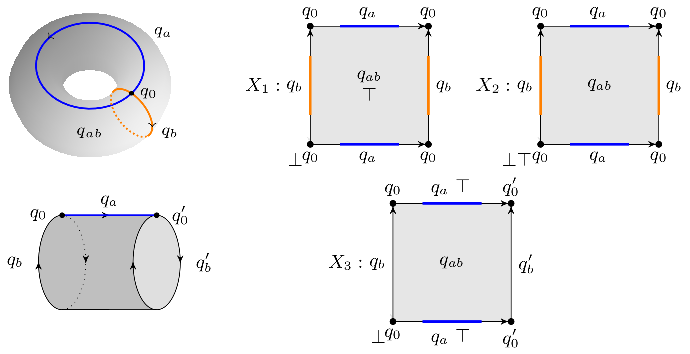
\includegraphics[width=0.95\linewidth,height=0.45\textheight,keepaspectratio]{graphic-09.pdf}\end{center}
 
Figure 8: Büchi $\omega$-HDAs (left) and unfolded views (right). See Ex. 18.\par
 
% END S3.F8
 
% BEGIN S3.SS2.p3
 
The language of a Büchi $\omega$-HDA $X$ is $L(X)={\{\mathsf{ev}(\alpha)\mathrel{\big{|}}\mathsf{src}(\alpha)\in\bot_{X}\text{ and }\mathsf{Inf}(\alpha)\cap\top_{X}\neq\emptyset\}}$ and we call Büchi $\omega$-regular such a language. Similarly, for a Muller $\omega$-HDA $Y$ we have ${L(Y)={\{\mathsf{ev}(\alpha)\mathrel{\big{|}}\mathsf{src}(\alpha)\in\bot_{Y}\text{ and }\mathsf{Inf}(\alpha)\in F_{Y}\}}}$ and we call Muller $\omega$-regular such a language. As in classical $\omega$-theory, a Büchi $\omega$-HDA $X_{B}$ can be seen as a Muller $\omega$-HDA $X_{M}$, where the acceptance condition is modified to $F_{X_{M}}={\{A\subseteq X\mathrel{\big{|}}A\cap\top_{X}\neq\emptyset\}}$. Hence Büchi $\omega$-regular languages are Muller $\omega$-regular. However, unlike HDAs over finite ipomsets we have:\par
 
% END S3.SS2.p3
 
% BEGIN Thmtheorem20
 
\par\medskip\noindent\textbf{Proposition 20.}\par
 
% BEGIN Thmtheorem20.p1
 
$\omega$-regular languages may not be down-closed.\par
 
% END Thmtheorem20.p1
 
% END Thmtheorem20
 
% BEGIN S3.SS2.SSS0.P0.SPx1
 
\par\medskip\noindent\textbf{Proof.}\par
 
% BEGIN S3.SS2.SSS0.P0.SPx1.p1
 
In the Büchi $\omega$-HDA $X_{1}$ of Ex. 18, we have $\left[\begin{smallmatrix}a\\
b\end{smallmatrix}\right]^{\omega}=\mathsf{ev}(q_{0},\mathrel{\nearrow^{ab}},q_{ab},\mathrel{\searrow_{ab}},q_{0},...)\in L(X_{1})$ (as it goes infinitely many times through $q_{ab}\in\top_{X_{1}}$). But $(ab)^{\omega}\sqsubseteq\left[\begin{smallmatrix}a\\
b\end{smallmatrix}\right]^{\omega}$, and the only $\omega$-track whose event is this $\omega$-ipomset is $(q_{0},\mathrel{\nearrow^{a}},q_{a},\mathrel{\searrow_{a}},q_{0},\mathrel{\nearrow^{b}},q_{b},\mathrel{\searrow_{b}},q_{0},...)$ which is not accepting. Thus $(ab)^{\omega}\not\in L(X_{1})$. The same can be done for the Muller $\omega$-HDA $X_{4}$ of Ex. 19. $\hfill\blacktriangleleft$\par
 
% END S3.SS2.SSS0.P0.SPx1.p1
 
% END S3.SS2.SSS0.P0.SPx1
 
% END S3.SS2
 
% END S3


% BEGIN S4
 
\par\medskip\noindent\textbf{4 $\omega$-rational languages}\par
 
% BEGIN S4.p1
 
We want to extend the notion of rationality to languages of interval $\omega$-ipomsets and capture the expressiveness of $\omega$-HDAs. Thus, we introduce a non-nested $\omega$-iteration over languages of finite interval ipomsets. On the other hand, the rational operations defined in [19] take subsumption into account. As languages of $\omega$-HDA are not down-closed, we cannot just extend these to $\omega$-ipomsets, but need to redefine them without subsumption closure.\par
 
% END S4.p1
 
% BEGIN S4.p2
 
We define the $\omega$-rational operations over $2^{\mathsf{iiPoms}^{\infty}}$ by:\par
  
\par\noindent  $\blacksquare$ 
% BEGIN S4.I1.i1.p1
 
For $(L,M)\subseteq{\mathsf{iiPoms}^{\infty}}\times{\mathsf{iiPoms}^{\infty}}$: $L+M=L\cup M$\par
 
% END S4.I1.i1.p1
 
 
\par\noindent  $\blacksquare$ 
% BEGIN S4.I1.i2.p1
 
For $(L,M)\subseteq\mathsf{iiPoms}\times{\mathsf{iiPoms}^{\infty}}$: $L*M=LM={\{P*Q\mathrel{\big{|}}P\in L,\,Q\in M,\,T_{P}\cong S_{Q}\}}$\par
 
% END S4.I1.i2.p1
 
 
\par\noindent  $\blacksquare$ 
% BEGIN S4.I1.i3.p1
 
For $L\subseteq\mathsf{iiPoms}$: $L^{+}=\bigcup_{n\geqslant 1}L^{n}$ (with $L^{1}=L$ and $L^{n+1}=L*L^{n}$)\par
 
% END S4.I1.i3.p1
 
 
\par\noindent  $\blacksquare$ 
% BEGIN S4.I1.i4.p1
 
For $L\subseteq\mathsf{iiPoms}$: $L^{\omega}={\{P_{1}*P_{2}*\dots\mathrel{\big{|}}\forall i,\,P_{i}\in L,T_{P_{i}}\cong S_{P_{i\text{+}1}}\text{ and }|{\{i:P_{i}\not\in\mathsf{Id}\}}|=+\infty\}}$\par
 
% END S4.I1.i4.p1
 
  
As in the finite case, the Kleene iteration is the non-empty + instead of ∗ because $L^{0}=\mathsf{Id}$ is not regular since it has infinite width. In addition, the operation $\parallel$ defined over languages of finite interval ipomsets (and over finite [28] and $\omega$-series-parallel pomsets [31]) is not used in our case. The reason is that it would typically not give interval $\omega$-ipomsets $(a^{\omega}\parallel b^{\omega}$ for example). In [19, Prop. 16], it is shown that $D\text{-}\mathcal{R}at$ may also be obtained from $\emptyset$ and $\Xi$ (the set of starters and terminators over $\Sigma$) using down-closed rational operations without $\|$. We define $\omega$-rational languages ${\mathcal{R}at}^{\infty}$ as the smallest set such that:\par
  
\par\noindent  $\blacksquare$ 
% BEGIN S4.I2.i1.p1
 
$\emptyset\in{\mathcal{R}at}^{\infty}$ and for $U\in\Xi$, ${\{U\}}\in{\mathcal{R}at}^{\infty}$;\par
 
% END S4.I2.i1.p1
 
 
\par\noindent  $\blacksquare$ 
% BEGIN S4.I2.i2.p1
 
if $L,M\in{\mathcal{R}at}^{\infty}$, then $L+M\in{\mathcal{R}at}^{\infty}$;\par
 
% END S4.I2.i2.p1
 
 
\par\noindent  $\blacksquare$ 
% BEGIN S4.I2.i3.p1
 
if $L,M\in{\mathcal{R}at}^{\infty}$ and $L\subseteq\mathsf{iPoms}$, then $L*M\in{\mathcal{R}at}^{\infty}$;\par
 
% END S4.I2.i3.p1
 
 
\par\noindent  $\blacksquare$ 
% BEGIN S4.I2.i4.p1
 
if $L\in{\mathcal{R}at}^{\infty}$ and $L\subseteq\mathsf{iPoms}$, then $L^{+}\in{\mathcal{R}at}^{\infty}$ and $L^{\omega}\in{\mathcal{R}at}^{\infty}$.\par
 
% END S4.I2.i4.p1
 
  
We will often use $U$ instead of ${\{U\}}$ for ease of reading. We define the width of a language $L$ by $\mathsf{wd}(L)=\mathsf{sup}{\{\mathsf{wd}(P)\mathrel{\big{|}}P\in L\}}$. As they are built inductively from $\Xi$, using finitely many $\omega$-rational operations, all $\omega$-rational languages have finite width.\par
 
% END S4.p2
 
% BEGIN Thmtheorem21
 
\par\medskip\noindent\textbf{Proposition 21.}\par
 
% BEGIN Thmtheorem21.p1
 
For $L\in{\mathcal{R}at}^{\infty}$, $\mathsf{wd}(L)<+\infty$.\par
 
% END Thmtheorem21.p1
 
% END Thmtheorem21
 
% BEGIN S4.p3
 
Thus, Prop. 21 and Lem. 4 imply that ${\mathcal{R}at}^{\infty}\subseteq 2^{\mathsf{iPoms}^{\infty}}$, that is, $\omega$-rational operations preserve validity. In addition, since $\Xi\subseteq\mathsf{iiPoms}$ and by Cor. 13, we have:\par
 
% END S4.p3
 
% BEGIN Thmtheorem22
 
\par\medskip\noindent\textbf{Proposition 22.}\par
 
% BEGIN Thmtheorem22.p1
 
For all $L\in{\mathcal{R}at}^{\infty}$, we have $L\subseteq{\mathsf{iiPoms}^{\infty}}$.\par
 
% END Thmtheorem22.p1
 
% END Thmtheorem22
 
% BEGIN S4.p4
 
We write ${\mathcal{R}at}^{\omega}={\mathcal{R}at}^{\infty}\cap 2^{\mathsf{iiPoms}^{\omega}}$ for $\omega$-rational languages, and $\mathcal{R}at={\mathcal{R}at}^{\infty}\cap 2^{\mathsf{iiPoms}}$ for finite ones. Note that $\mathcal{R}at$ is not the class of rational languages defined in [19] (that we denote $D\text{-}\mathcal{R}at$ for down-closed rational). For example, ${\{\left[\begin{smallmatrix}a\vbox{\hbox{\tiny$\bullet$}}\\
b\vbox{\hbox{\tiny$\bullet$}}\end{smallmatrix}\right]\}}*{\{\left[\begin{smallmatrix}\vbox{\hbox{\tiny$\bullet$}}a\\
\vbox{\hbox{\tiny$\bullet$}}b\end{smallmatrix}\right]\}}={\{\left[\begin{smallmatrix}a\\
b\end{smallmatrix}\right]\}}\in\mathcal{R}at$ as the gluing of a starter and a terminator, but is not in $D\text{-}\mathcal{R}at$ (because not down-closed). We show in Prop. 36 that up to down-closure, both notions are equivalent in the finite case.\par
 
% END S4.p4
 
% END S4


% BEGIN S5
 
\par\medskip\noindent\textbf{5 $\omega$-rationality vs. $\omega$-regularity}\par
 
% BEGIN S5.p1
 
In this section, we explore the connections between $\omega$-rationality and $\omega$-regularity. We show that $\omega$-regular languages are $\omega$-rational. The proof relies on a type of classical $\omega$-automata derived from $\omega$-HDAs called ST-automata. On the other hand, the opposite does not hold. Indeed, we show that Muller acceptance is more expressive than Büchi acceptance and that there are $\omega$-rational languages that are not Muller $\omega$-regular.\par
 
% END S5.p1
 
% BEGIN S5.SS1
 
\par\medskip\noindent\textbf{5.1 ST-automata for $\omega$-HDA}\par
 
% BEGIN S5.SS1.p1
 
An ST-automaton is a plain ($\omega$-)automaton over $\Xi$, with an additional labeling of states, that can produce ($\omega$-)iipomsets if the letters are glued. It especially can mimic the behavior of an ($\omega$-)HDA with a canonical translation. We use here the most recent definition of these objects, introduced in [4], which subsumes other variants that have been used in [19, 7, 2, 3, 8, 17, 16].\par
 
% END S5.SS1.p1
 
% BEGIN S5.SS1.p2
 
We let $\overline{\Xi}=(\overline{\Xi},{\cdot},\varepsilon)$ denote the free monoid on $\overline{\Xi}=\Xi$ seen as an alphabet, using concatenation instead of gluing and $\varepsilon$ for the empty word (which is different from the letter $\mathsf{id}_{\emptyset}\in\overline{\Xi}$).\par
 
% END S5.SS1.p2
 
% BEGIN S5.SS1.p3
 
An ST-automaton $A$ is a finite labeled automaton $(Q,E,I,F,\lambda)$ over the (infinite) alphabet $\overline{\Xi}$, where $Q$ is the set of states, $E\subseteq Q\times(\overline{\Xi}\setminus\mathsf{Id})\times Q$ is the set of transitions, $I\subseteq Q$ are the initial states, $F$ is an acceptance condition and $\lambda:Q\rightarrow\square$ is a labeling of states that is coherent with $E$, meaning that for all $(p,{\vphantom{U}}_{S}U_{T},q)\in E,\,\lambda(p)=S$ and $\lambda(q)=T$.\par
 
% END S5.SS1.p3
 
% BEGIN S5.SS1.p4
 
A path $\pi=(q_{0},e_{0},q_{1},e_{1},\dots,e_{n-1},q_{n})$ in an ST-automaton $A$ is an alternation of states and transitions such that ${e_{i}=(q_{i},P_{i},q_{i+1})\in E}$. Its label is $l(\pi)=\mathsf{id}_{\lambda(q_{0})}\cdot P_{0}\cdot\mathsf{id}_{\lambda(q_{1})}\cdot$ $\ldots\cdot P_{n-1}\cdot\mathsf{id}_{\lambda(q_{n})}$ seen as a word. We say that $\pi$ is accepting if $q_{0}\in I$ and $q_{n}\in F$. The language of an ST-automaton $A$, denoted $L(A)$, is the set of labels of its accepting paths. The same can be done for $\omega$-paths, which are accepted according to a Büchi or Muller condition.\par
 
% END S5.SS1.p4
 
% BEGIN Thmtheorem23
 
\par\medskip\noindent\textbf{$\blacktriangleright$ Remark 23.}\par
 
% BEGIN Thmtheorem23.p1
 
Path labels of ST-automata are elements of $\mathsf{Id}\cdot(\overline{\Xi}\cdot\mathsf{Id})^{*}$ (or $\mathsf{Id}\cdot(\overline{\Xi}\cdot\mathsf{Id})^{\omega}$ in the infinite case). In particular, the labeling of states and their consideration in the path labels forbid to have the empty word $\varepsilon$ as the label of a path. Note also that labels of states are not used twice: given $\pi_{1}=(q_{0},e_{0},\dots,e_{i-1},q_{i})$ and $\pi_{2}=(q_{i},e_{i},,\dots,e_{n-1},q_{n})$, we have $l(\pi_{1})\cdot l(\pi_{2})=\mathsf{id}_{\lambda(q_{0})}\cdot P_{0}\cdot\mathsf{id}_{\lambda(q_{1})}\cdot\ldots\cdot P_{i-1}\cdot\mathsf{id}_{\lambda(q_{i})}\cdot P_{i+1}\cdot\ldots\cdot P_{n-1}\cdot\mathsf{id}_{\lambda(q_{n})}$. We are thus only able to concatenate $l(\pi_{1})$ and $l(\pi_{2})$ if the end of $\pi_{1}$ has the same label as the start of $\pi_{2}$. We will consider ($\omega$-)rational expressions of ST-automata as classical ($\omega$-)rational expressions, the only difference being that the concatenation operator behaves as stated above.\par
 
% END Thmtheorem23.p1
 
% END Thmtheorem23
 
% BEGIN S5.SS1.p5
 
In the following, we build an ST-automaton $ST(X)$ from an ($\omega$-)HDA $X$, following [4]. The intuition is that each cell (of any dimension) becomes a state, and for each upstep $(p=\delta_{A}^{0}(q),{\mathrel{\nearrow^{A}}},q)$ resp. downstep $(p,\mathrel{\searrow_{B}},\delta_{B}^{1}(p)=q)$ in $X$, a transition is introduced from the state corresponding to $p$ to the one corresponding to $q$, labeled with ${}_{A\!}{\uparrow}{\mathsf{ev}(q)}$ resp. ${\mathsf{ev}(p)}{\downarrow}_{B}$), to mimic the behavior of the HDA. More formally, for an HDA $(X,\bot_{X},F_{X})$, we associate the ST-automaton $ST(X)=(Q,E,I,F,\lambda)$ with:\par
  
\par\noindent  $\blacksquare$ 
% BEGIN S5.I1.i1.p1
 
$Q=X$, $I=\bot_{X}$, $F=F_{X}$, $\lambda=\mathsf{ev}$,\par
 
% END S5.I1.i1.p1
 
 
\par\noindent  $\blacksquare$ 
% BEGIN S5.I1.i2.p1
 
$E={\{(\delta_{A}^{0}(q),{}_{A\!}{\uparrow}{\mathsf{ev}(q)},q)\mathrel{\big{|}}A\subseteq\mathsf{ev}(q)\}}\cup{\{(q,{\mathsf{ev}(q)}{\downarrow}_{A},\delta_{A}^{1}(q))\mathrel{\big{|}}A\subseteq\mathsf{ev}(q)\}}$.\par
 
% END S5.I1.i2.p1
 
  
By construction, there is a one-to-one correspondence between tracks in $X$ and paths in $ST(X)$: with a track $\alpha=(q_{0},\varphi_{0},q_{1},...)$ of $X$ we associate the path $ST(\alpha)=(q_{0},e_{0},q_{1},...)$ of $ST(X)$ such that\par
  
\par\noindent  $\blacksquare$ 
% BEGIN S5.I2.i1.p1
 
$(q_{i},\varphi_{i},q_{i\text{+}1})=(\delta_{A_{i}}^{0}(q_{i\text{+}1}),\mathrel{\nearrow^{A_{i}}},q_{i\text{+}1})\Rightarrow A_{i}\subseteq\mathsf{ev}(q_{i\text{+}1})$, $e_{i}=(q_{i},{}_{A_{i}\!}{\uparrow}{\mathsf{ev}(q_{i\text{+}1})},q_{i\text{+}1})\in E$\par
 
% END S5.I2.i1.p1
 
 
\par\noindent  $\blacksquare$ 
% BEGIN S5.I2.i2.p1
 
$(q_{i},\varphi_{i},q_{i\text{+}1})=(q_{i},\mathrel{\searrow_{A_{i}}},\delta_{A_{i}}^{1}(q_{i}))\Rightarrow A_{i}\subseteq\mathsf{ev}(q_{i})$, $e_{i}=(q_{i},{\mathsf{ev}(q_{i})}{\downarrow}_{A_{i}},q_{i\text{+}1})\in E$\par
 
% END S5.I2.i2.p1
 
  
This proves the following lemma:\par
 
% END S5.SS1.p5
 
% BEGIN Thmtheorem24
 
\par\medskip\noindent\textbf{Lemma 24.}\par
 
% BEGIN Thmtheorem24.p1
 
A track $\alpha$ is accepting in $X$ if and only if $ST(\alpha)$ is accepting in $ST(X)$.\par
 
% END Thmtheorem24.p1
 
% END Thmtheorem24
 
% BEGIN S5.F9

\begin{center}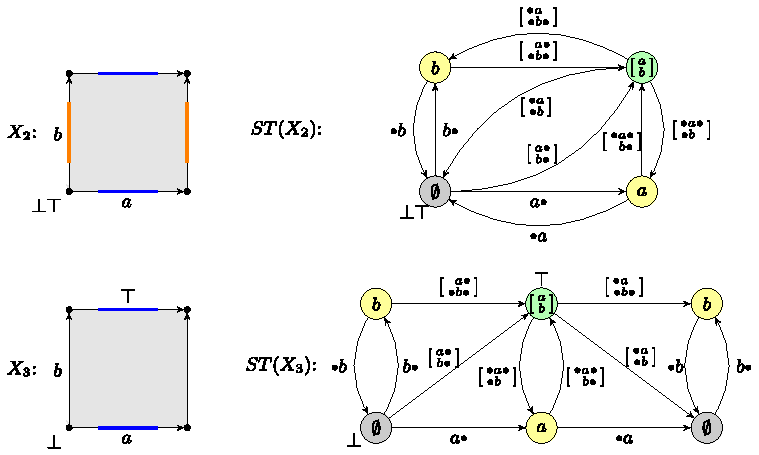
\includegraphics[width=0.95\linewidth,height=0.45\textheight,keepaspectratio]{graphic-10.pdf}\end{center}
 
Figure 9: ST-automata of $X_{2}$ and $X_{3}$ of Ex. 18. Cells of dimension 0 are in gray, dimension 1 in yellow, and dimension 2 in green.\par
 
% END S5.F9
 
% BEGIN S5.SS1.p6
 
Since the labeling $\lambda$ is coherent with $E$, a word produced by an ST-automaton $A$ is coherent in the sense that if $P_{1}\cdot P_{2}\cdot\ldots$ is the label of a path in $A$, then $T_{P_{i}}\cong S_{P_{i\text{+}1}}$ for all $i\geqslant 0$ (and thus it can be seen as the gluing of starters and terminators). To be more precise, the set of coherent finite words over $\overline{\Xi}$ is denoted $\mathsf{Coh}^{+}(\overline{\Xi})={\{U_{1}\cdot\ldots\cdot U_{n}\mathrel{\big{|}}U_{i}\in\overline{\Xi},\ T_{U_{i}}\cong S_{U_{i\text{+}1}}\}}$.\par
 
% END S5.SS1.p6
 
% BEGIN S5.SS1.p7
 
For $\omega$-words we denote by $\mathsf{Coh}^{\omega}(\overline{\Xi})$ the set of coherent infinite words over $\overline{\Xi}$, defined by\par
    \[{\mathsf{Coh}^{\omega}(\overline{\Xi})={\{U_{1}\cdot U_{2}\cdot\ldots\mathrel{\big{|}}U_{i}\in\overline{\Xi},\ \#{\{i:U_{i}\not\in\mathsf{Id}\}}=+\infty\text{ and }T_{U_{i}}=S_{U_{i\text{+}1}}\}}}\]    
and as usual we write $\mathsf{Coh}^{\infty}(\overline{\Xi})=\mathsf{Coh}^{+}(\overline{\Xi})\cup\mathsf{Coh}^{\omega}(\overline{\Xi})$.\par
 
% END S5.SS1.p7
 
% BEGIN Thmtheorem25
 
\par\medskip\noindent\textbf{Lemma 25.}\par
 
% BEGIN Thmtheorem25.p1
 
Let $A$ be an ST-automaton.\par
  
\par\noindent  $\blacksquare$ 
% BEGIN S5.I3.i1.p1
 
If $A$ accepts finite words then $L(A)\subseteq\mathsf{Coh}^{+}(\overline{\Xi})$.\par
 
% END S5.I3.i1.p1
 
 
\par\noindent  $\blacksquare$ 
% BEGIN S5.I3.i2.p1
 
If $A$ accepts infinite words then $L(A)\subseteq\mathsf{Coh}^{\omega}(\overline{\Xi})$.\par
 
% END S5.I3.i2.p1
 
  
% END Thmtheorem25.p1
 
% END Thmtheorem25
 
% BEGIN S5.SS1.p8
 
Thus, one can “glue” words accepted by an ST-automaton to obtain an ($\omega$-)iipomset. Let $\Psi\colon\mathsf{Coh}^{\infty}(\overline{\Xi})\to{\mathsf{iPoms}^{\infty}}$ be the gluing function defined by $\Psi(P_{1}\cdot P_{2}\cdot\dots)=P_{1}*P_{2}*\dots$. For a set $L\subseteq\mathsf{Coh}^{\infty}(\overline{\Xi})$, we also define $\Psi(L)={\{\Psi(P)\mathrel{\big{|}}P\in L\}}$. In [4], the authors show the following for ST-automata derived from HDAs over finite iipomsets:\par
 
% END S5.SS1.p8
 
% BEGIN Thmtheorem26
 
\par\medskip\noindent\textbf{Proposition 26 ([4]).}\par
 
% BEGIN Thmtheorem26.p1
 
For any HDA $X$, $L(X)=\Psi(L(ST(X)))$.\par
 
% END Thmtheorem26.p1
 
% END Thmtheorem26
 
% BEGIN S5.SS1.p9
 
We show that the proposition holds also for $\omega$-HDAs. First, since the labeling of states is coherent with the transitions, we have the following by applying definitions.\par
 
% END S5.SS1.p9
 
% BEGIN Thmtheorem27
 
\par\medskip\noindent\textbf{Lemma 27.}\par
 
% BEGIN Thmtheorem27.p1
 
For all $\omega$-tracks $\alpha$ of $X$, we have $\mathsf{ev}(\alpha)=\Psi(l(ST(\alpha))$.\par
 
% END Thmtheorem27.p1
 
% END Thmtheorem27
 
% BEGIN S5.SS1.p10
 
We can now show the $\omega$-equivalent of Prop. 26, by combining Lem. 24 and Lem. 27:\par
 
% END S5.SS1.p10
 
% BEGIN Thmtheorem28
 
\par\medskip\noindent\textbf{Proposition 28.}\par
 
% BEGIN Thmtheorem28.p1
 
For any (Büchi or Muller) $\omega$-HDA $X$, $L(X)=\Psi(L(ST(X)))$.\par
 
% END Thmtheorem28.p1
 
% END Thmtheorem28
 
% END S5.SS1
 
% BEGIN S5.SS2
 
\par\medskip\noindent\textbf{5.2 $\omega$-HDAs are $\omega$-rational}\par
 
% BEGIN S5.SS2.p1
 
The formalism of ST-automata provides a strong tool for HDAs. It allows to use classical theorems of $\omega$-automata. This helps in particular to show that $\omega$-regular languages are $\omega$-rational as we will see in this section.\par
 
% END S5.SS2.p1
 
% BEGIN S5.SS2.p2
 
Indeed, the language of any ST-automaton $A$ is also the one of a rational expression $e_{A}$, using the operations $+,.\,,^{*}$ and letters $U_{i}\in\overline{\Xi}$. Similarly, given an ST-automaton $A^{\prime}$ over infinite words, one can effectively build an equivalent $\omega$-rational expression $e_{A^{\prime}}$ [36].\par
 
% END S5.SS2.p2
 
% BEGIN S5.SS2.p3
 
A ($\omega$-)rational expression is said positive if it has no occurrences of ∗ and $\varepsilon$. Since ST-automata do not accept $\varepsilon$, ST-automata languages can be expressed by positive expressions:\par
 
% END S5.SS2.p3
 
% BEGIN Thmtheorem29
 
\par\medskip\noindent\textbf{Lemma 29.}\par
 
% BEGIN Thmtheorem29.p1
 
Any rational expression $e$ of an ST-automaton can be transformed into a positive rational expression $\overline{e}$ such that $\mathcal{L}(e)=\mathcal{L}(\overline{e})$.\par
 
% END Thmtheorem29.p1
 
% END Thmtheorem29
 
% BEGIN S5.SS2.p4
 
We define inductively a function $\Psi^{\prime}$ transforming a positive rational expression over $\overline{\Xi}$ into a set of ipomsets in the usual way by replacing $\cdot$ by $*$. We directly have:\par
 
% END S5.SS2.p4
 
% BEGIN Thmtheorem30
 
\par\medskip\noindent\textbf{Lemma 30.}\par
 
% BEGIN Thmtheorem30.p1
 
Let $e(U_{1},...,U_{n})$ be a positive rational expression over $\overline{\Xi}$.\par
  
\par\noindent  $\blacksquare$ 
% BEGIN S5.I4.i1.p1
 
If $e$ is rational, then $\Psi^{\prime}(e)\in\mathcal{R}at$.\par
 
% END S5.I4.i1.p1
 
 
\par\noindent  $\blacksquare$ 
% BEGIN S5.I4.i2.p1
 
If $e$ is $\omega$-rational, then $\Psi^{\prime}(e)\in{\mathcal{R}at}^{\omega}$.\par
 
% END S5.I4.i2.p1
 
  
% END Thmtheorem30.p1
 
% END Thmtheorem30
 
% BEGIN S5.SS2.p5
 
In addition, we can show by induction that $\Psi^{\prime}$ preserves languages.\par
 
% END S5.SS2.p5
 
% BEGIN Thmtheorem31
 
\par\medskip\noindent\textbf{Lemma 31.}\par
 
% BEGIN Thmtheorem31.p1
 
If $e$ is an ($\omega$-)rational expression over $\overline{\Xi}$, then $\Psi^{\prime}(e)=\Psi(\mathcal{L}(e))$\par
 
% END Thmtheorem31.p1
 
% END Thmtheorem31
 
% BEGIN S5.SS2.p6
 
Thus, languages of ST-automata are rational:\par
 
% END S5.SS2.p6
 
% BEGIN Thmtheorem32
 
\par\medskip\noindent\textbf{Lemma 32.}\par
 
% BEGIN Thmtheorem32.p1
 
Let $A$ be an ST-automaton.\par
  
\par\noindent  $\blacksquare$ 
% BEGIN S5.I5.i1.p1
 
If $A$ accepts finite words, then $\Psi(L(A))\in\mathcal{R}at$.\par
 
% END S5.I5.i1.p1
 
 
\par\noindent  $\blacksquare$ 
% BEGIN S5.I5.i2.p1
 
If $A$ accepts infinite words, then $\Psi(L(A))\in{\mathcal{R}at}^{\omega}$.\par
 
% END S5.I5.i2.p1
 
  
% END Thmtheorem32.p1
 
% END Thmtheorem32
 

% BEGIN Thmtheorem33
 
\par\medskip\noindent\textbf{Theorem 33.}\par
 
% BEGIN Thmtheorem33.p1
 
Büchi and Muller $\omega$-regular languages are $\omega$-rational.\par
 
% END Thmtheorem33.p1
 
% END Thmtheorem33

 

% BEGIN S5.SS2.SSS0.P0.SPx1
 
\par\medskip\noindent\textbf{Proof.}\par
 
% BEGIN S5.SS2.SSS0.P0.SPx1.p1
 
Let $(X,\bot_{X},F_{X})$ be a Büchi or Muller $\omega$-HDA. By definition of $\omega$-HDAs, $X$ is finite, hence so is its ST-automaton $ST(X)$. By Prop. 28, $L(X)=\Psi(L(ST(X)))$, and by Lem. 32, $\Psi(L(ST(X)))\in{\mathcal{R}at}^{\omega}$, thus all $\omega$-regular languages are $\omega$-rational. $\hfill\blacktriangleleft$\par
 
% END S5.SS2.SSS0.P0.SPx1.p1
 
% BEGIN S5.SS2.SSS0.P0.SPx1.p2
 
As a corollary of the above and Prop. 22 we have:\par
 
% END S5.SS2.SSS0.P0.SPx1.p2
 
% BEGIN Thmtheorem34
 
\par\medskip\noindent\textbf{Corollary 34.}\par
 
% BEGIN Thmtheorem34.p1
 
If $L$ is an $\omega$-regular language, then $\mathsf{wd}(L)<+\infty$ and $L\subseteq{\mathsf{iiPoms}^{\omega}}$.\par
 
% END Thmtheorem34.p1
 
% END Thmtheorem34
 
% BEGIN Thmtheorem35
 
\par\medskip\noindent\textbf{Example 35.}\par
 
% BEGIN Thmtheorem35.p1
 
In Fig. 9 are represented two $\omega$-HDAs with their corresponding ST-automata. From this we can directly compute their language in $\overline{\Xi}^{\omega}$ (we omit the letters in $\mathsf{Id}$), and then use $\Psi$ to compute the languages of the original Büchi $\omega$-HDAs:\par
 
% END Thmtheorem35.p1
 
% BEGIN Thmtheorem35.p2
 
\begin{center}\resizebox{\linewidth}{!}{$\begin{aligned}\displaystyle L(ST(X_{2}))= & \displaystyle\Big{(}a\vbox{\hbox{\tiny$\bullet$}}\cdot\vbox{\hbox{\tiny$\bullet$}}a+b\vbox{\hbox{\tiny$\bullet$}}\cdot\vbox{\hbox{\tiny$\bullet$}}b+(a\vbox{\hbox{\tiny$\bullet$}}\cdot\left[\begin{smallmatrix}\vbox{\hbox{\tiny$\bullet$}}a\vbox{\hbox{\tiny$\bullet$}}\\
\hphantom{\vbox{\hbox{\tiny$\bullet$}}}b\vbox{\hbox{\tiny$\bullet$}}\end{smallmatrix}\right]+\left[\begin{smallmatrix}a\vbox{\hbox{\tiny$\bullet$}}\\
b\vbox{\hbox{\tiny$\bullet$}}\end{smallmatrix}\right]+b\vbox{\hbox{\tiny$\bullet$}}\cdot\left[\begin{smallmatrix}\hphantom{\vbox{\hbox{\tiny$\bullet$}}}a\vbox{\hbox{\tiny$\bullet$}}\\
\vbox{\hbox{\tiny$\bullet$}}b\vbox{\hbox{\tiny$\bullet$}}\end{smallmatrix}\right])\cdot(\left[\begin{smallmatrix}\vbox{\hbox{\tiny$\bullet$}}a\vbox{\hbox{\tiny$\bullet$}}\\
\vbox{\hbox{\tiny$\bullet$}}b\hphantom{\vbox{\hbox{\tiny$\bullet$}}}\end{smallmatrix}\right]\cdot\left[\begin{smallmatrix}\vbox{\hbox{\tiny$\bullet$}}a\vbox{\hbox{\tiny$\bullet$}}\\
\hphantom{\vbox{\hbox{\tiny$\bullet$}}}b\vbox{\hbox{\tiny$\bullet$}}\end{smallmatrix}\right]+\left[\begin{smallmatrix}\vbox{\hbox{\tiny$\bullet$}}a\hphantom{\vbox{\hbox{\tiny$\bullet$}}}\\
\vbox{\hbox{\tiny$\bullet$}}b\vbox{\hbox{\tiny$\bullet$}}\end{smallmatrix}\right]\cdot\left[\begin{smallmatrix}\hphantom{\vbox{\hbox{\tiny$\bullet$}}}a\vbox{\hbox{\tiny$\bullet$}}\\
\vbox{\hbox{\tiny$\bullet$}}b\vbox{\hbox{\tiny$\bullet$}}\end{smallmatrix}\right])^{*}\\\displaystyle\cdot(\left[\begin{smallmatrix}\vbox{\hbox{\tiny$\bullet$}}a\vbox{\hbox{\tiny$\bullet$}}\\
\vbox{\hbox{\tiny$\bullet$}}b\hphantom{\vbox{\hbox{\tiny$\bullet$}}}\end{smallmatrix}\right]\cdot\vbox{\hbox{\tiny$\bullet$}}a+\left[\begin{smallmatrix}\vbox{\hbox{\tiny$\bullet$}}a\\
\vbox{\hbox{\tiny$\bullet$}}b\end{smallmatrix}\right]+\left[\begin{smallmatrix}\vbox{\hbox{\tiny$\bullet$}}a\hphantom{\vbox{\hbox{\tiny$\bullet$}}}\\
\vbox{\hbox{\tiny$\bullet$}}b\vbox{\hbox{\tiny$\bullet$}}\end{smallmatrix}\right]\cdot\vbox{\hbox{\tiny$\bullet$}}b)\Big{)}^{\omega}\\\displaystyle L(ST(X_{3}))= & \displaystyle(b\vbox{\hbox{\tiny$\bullet$}}\cdot\vbox{\hbox{\tiny$\bullet$}}b)^{*}\cdot(a\vbox{\hbox{\tiny$\bullet$}}\cdot\left[\begin{smallmatrix}\vbox{\hbox{\tiny$\bullet$}}a\vbox{\hbox{\tiny$\bullet$}}\\
\hphantom{\vbox{\hbox{\tiny$\bullet$}}}b\vbox{\hbox{\tiny$\bullet$}}\end{smallmatrix}\right]+b\vbox{\hbox{\tiny$\bullet$}}\cdot\left[\begin{smallmatrix}\hphantom{\vbox{\hbox{\tiny$\bullet$}}}a\vbox{\hbox{\tiny$\bullet$}}\\
\vbox{\hbox{\tiny$\bullet$}}b\vbox{\hbox{\tiny$\bullet$}}\end{smallmatrix}\right]+\left[\begin{smallmatrix}a\vbox{\hbox{\tiny$\bullet$}}\\
b\vbox{\hbox{\tiny$\bullet$}}\end{smallmatrix}\right])\cdot(\left[\begin{smallmatrix}\vbox{\hbox{\tiny$\bullet$}}a\vbox{\hbox{\tiny$\bullet$}}\\
\vbox{\hbox{\tiny$\bullet$}}b\hphantom{\vbox{\hbox{\tiny$\bullet$}}}\end{smallmatrix}\right]\cdot\left[\begin{smallmatrix}\vbox{\hbox{\tiny$\bullet$}}a\vbox{\hbox{\tiny$\bullet$}}\\
\hphantom{\vbox{\hbox{\tiny$\bullet$}}}b\vbox{\hbox{\tiny$\bullet$}}\end{smallmatrix}\right])^{\omega}\end{aligned}$}\end{center}
 
Languages in $\mathsf{Coh}^{\omega}(\overline{\Xi})$ can be turned into the language of the original HDA using the function $\Psi$ and Prop. 26. We just replace the occurrences of $A^{*}$ by $A^{+}+\varepsilon$ and develop the expression to avoid the word $\varepsilon$, then remove multiple occurrences of the same ipomset in unions:\par
  
\par\noindent  $\blacksquare$ 
% BEGIN S5.I6.i1.p1
 
$L(X_{2})=\Psi(L(ST(X_{2})))=(a+b+\left[\begin{smallmatrix}a\\
b\end{smallmatrix}\right]+\left[\begin{smallmatrix}a\vbox{\hbox{\tiny$\bullet$}}\\
b\vbox{\hbox{\tiny$\bullet$}}\end{smallmatrix}\right]*(\left[\begin{smallmatrix}\vbox{\hbox{\tiny$\bullet$}}a\vbox{\hbox{\tiny$\bullet$}}\\
\vbox{\hbox{\tiny$\bullet$}}bb\vbox{\hbox{\tiny$\bullet$}}\end{smallmatrix}\right]+\left[\begin{smallmatrix}\vbox{\hbox{\tiny$\bullet$}}aa\vbox{\hbox{\tiny$\bullet$}}\\
\vbox{\hbox{\tiny$\bullet$}}b\vbox{\hbox{\tiny$\bullet$}}\end{smallmatrix}\right])^{+}*\left[\begin{smallmatrix}\vbox{\hbox{\tiny$\bullet$}}a\\
\vbox{\hbox{\tiny$\bullet$}}b\end{smallmatrix}\right])^{\omega}$\par
 
% END S5.I6.i1.p1
 
 
\par\noindent  $\blacksquare$ 
% BEGIN S5.I6.i2.p1
 
$L(X_{3})=\Psi(L(ST(X_{3})))=b^{+}*\left[\begin{smallmatrix}a\vbox{\hbox{\tiny$\bullet$}}\\
b\vbox{\hbox{\tiny$\bullet$}}\end{smallmatrix}\right]*\left[\begin{smallmatrix}\vbox{\hbox{\tiny$\bullet$}}a\vbox{\hbox{\tiny$\bullet$}}\\
\vbox{\hbox{\tiny$\bullet$}}bb\vbox{\hbox{\tiny$\bullet$}}\end{smallmatrix}\right]^{\omega}+\left[\begin{smallmatrix}a\vbox{\hbox{\tiny$\bullet$}}\\
b\vbox{\hbox{\tiny$\bullet$}}\end{smallmatrix}\right]*\left[\begin{smallmatrix}\vbox{\hbox{\tiny$\bullet$}}a\vbox{\hbox{\tiny$\bullet$}}\\
\vbox{\hbox{\tiny$\bullet$}}bb\vbox{\hbox{\tiny$\bullet$}}\end{smallmatrix}\right]^{\omega}$\par
 
% END S5.I6.i2.p1
 
  
% END Thmtheorem35.p2
 
% END Thmtheorem35
 
% BEGIN S5.SS2.SSS0.P0.SPx1.p3
 
As we saw in the previous section, our definition of rational operations is different from the original one [19] since we do not take subsumption closure into account. Nevertheless:\par
 
% END S5.SS2.SSS0.P0.SPx1.p3
 
% BEGIN Thmtheorem36
 
\par\medskip\noindent\textbf{Proposition 36.}\par
 
% BEGIN Thmtheorem36.p1
 
$\mathcal{R}at\mathord{\downarrow}=D\text{-}\mathcal{R}at$.\par
 
% END Thmtheorem36.p1
 
% END Thmtheorem36
 
% END S5.SS2.SSS0.P0.SPx1

 
% BEGIN S5.SS2.SSS0.P0.SPx2
 
\par\medskip\noindent\textbf{Proof.}\par
 
% BEGIN S5.SS2.SSS0.P0.SPx2.p1
 
The inclusion $\mathcal{R}at\mathord{\downarrow}\subseteq D\text{-}\mathcal{R}at$ is done by induction. The other follows from Lem. 32 and the fact that languages of $D\text{-}\mathcal{R}at$ are closed under subsumption (see App. B for details). $\hfill\blacktriangleleft$\par
 
% END S5.SS2.SSS0.P0.SPx2.p1
 
% END S5.SS2.SSS0.P0.SPx2
 
% END S5.SS2
 
% BEGIN S5.SS3
 
\par\medskip\noindent\textbf{5.3 Muller vs Büchi vs $\omega$-rational}\par
 
% BEGIN S5.SS3.p1
 
In the classical $\omega$-theory, rational languages are as expressive as Muller and Büchi automata. For $\omega$-HDA, these are no longer true. We describe and prove here some differences:\par
 
% END S5.SS3.p1
 
% BEGIN Thmtheorem37
 
\par\medskip\noindent\textbf{Theorem 37.}\par
 
% BEGIN Thmtheorem37.p1
 
The Muller $\omega$-regular class is strictly bigger than the Büchi $\omega$-regular class.\par
 
% END Thmtheorem37.p1
 
% END Thmtheorem37
 
% BEGIN S5.SS3.SSS0.P0.SPx1
 
\par\medskip\noindent\textbf{Proof.}\par
 
% BEGIN S5.SS3.SSS0.P0.SPx1.p1
 
As for the classical $\omega$-theory, Büchi $\omega$-regular languages are Muller $\omega$-regular.\par
 
% END S5.SS3.SSS0.P0.SPx1.p1
 
% BEGIN S5.SS3.SSS0.P0.SPx1.p2
 
However, the converse is false. Take the Muller $\omega$-HDA $X_{4}$ of Ex. 19. The only cycle (up to shift) using only states of $F_{X_{4}}$ is $(q_{0},\mathrel{\nearrow^{ab}},q_{ab},\mathrel{\searrow_{ab}},q_{0},...)$, so the language of $X_{4}$ is such that every accepted $\omega$-ipomset ends by $\left[\begin{smallmatrix}a\\
b\end{smallmatrix}\right]^{\omega}$. Assume that there is a Büchi $\omega$-HDA $Y$ that recognizes $L(X_{4})$. Let $\alpha$ be an accepting $\omega$-track of $Y$, which exists because $L(X_{4})\neq\emptyset$. We have $\mathsf{ev}(\alpha)=A*\left[\begin{smallmatrix}a\\
b\end{smallmatrix}\right]^{\omega}$ for some $A\in\mathsf{iiPoms}$. So $\alpha$ goes through $Y[\left[\begin{smallmatrix}a\\
b\end{smallmatrix}\right]]$ an infinite number of times. However $Y$ is finite, so there is $p\in Y[\left[\begin{smallmatrix}a\\
b\end{smallmatrix}\right]]$ such that $\alpha$ goes through $p$ an infinite number of times. Thus there is a subtrack $\alpha_{p}:=(\delta^{0}_{ab}(p),\mathrel{\nearrow^{ab}},p,\mathrel{\searrow_{ab}},\delta^{1}_{ab}(p))$ which appears an infinite number of times in $\alpha$. (It may be a track equivalent to it, but as there is a finite number of them, it suffices to choose one of them that is used an infinite number of times.) As $Y$ is a precubical set, we can define the track $\alpha^{\prime}_{p}=(\delta^{0}_{ab}(p),\mathrel{\nearrow^{a}},\delta^{0}_{b}(p),\mathrel{\searrow_{a}},\delta^{1}_{a}(\delta^{0}_{b}(p)),\mathrel{\nearrow^{b}},\delta^{1}_{a}(p),\mathrel{\searrow_{b}},\delta^{1}_{ab}(p))$ with label $ab$, and then replace one in two occurrences of $\alpha_{p}$ by $\alpha^{\prime}_{p}$. The cells visited an infinite number of times by $\alpha$ are still visited an infinite number of times, hence the new $\omega$-track is also accepting. However, its label does not end by $\left[\begin{smallmatrix}a\\
b\end{smallmatrix}\right]^{\omega}$ because $ab$ appears an infinite number of times. So $L(X_{4})$ is not Büchi $\omega$-regular. $\hfill\blacktriangleleft$\par
 
% END S5.SS3.SSS0.P0.SPx1.p2
 
% BEGIN Thmtheorem38
 
\par\medskip\noindent\textbf{Theorem 38.}\par
 
% BEGIN Thmtheorem38.p1
 
Some languages of ${\mathcal{R}at}^{\omega}$ cannot be expressed by Muller $\omega$-HDA.\par
 
% END Thmtheorem38.p1
 
% END Thmtheorem38
 
% END S5.SS3.SSS0.P0.SPx1
 
% BEGIN S5.SS3.SSS0.P0.SPx2
 
\par\medskip\noindent\textbf{Proof.}\par
 
% BEGIN S5.SS3.SSS0.P0.SPx2.p1
 
Let $L_{r}=(\left[\begin{smallmatrix}a\vbox{\hbox{\tiny$\bullet$}}\\
b\vbox{\hbox{\tiny$\bullet$}}\end{smallmatrix}\right]*\left[\begin{smallmatrix}\vbox{\hbox{\tiny$\bullet$}}a\\
\vbox{\hbox{\tiny$\bullet$}}b\end{smallmatrix}\right])^{\omega}=\left[\begin{smallmatrix}a\\
b\end{smallmatrix}\right]^{\omega}\in{\mathcal{R}at}^{\omega}$. Suppose that $(X,\bot_{X},F_{X})$ is a Muller $\omega$-HDA such that $L(X)=L_{r}$. An accepting $\omega$-track $\alpha$ (with label $\mathsf{ev}(\alpha)=\left[\begin{smallmatrix}a\\
b\end{smallmatrix}\right]^{\omega}$) in $X$ must start by a track (equivalent to) $\alpha_{p}:=(\delta^{0}_{ab}(p),\mathrel{\nearrow^{ab}},p,\mathrel{\searrow_{ab}},\delta^{1}_{ab}(p))$ with $p\in X[\left[\begin{smallmatrix}a\\
b\end{smallmatrix}\right]]$. As $X$ is a precubical set, $\alpha^{\prime}_{p}=(\delta^{0}_{ab}(p),\mathrel{\nearrow^{a}},\delta^{0}_{b}(p),\mathrel{\searrow_{a}},\delta^{1}_{a}(\delta^{0}_{b}(p)),\mathrel{\nearrow^{b}},\delta^{1}_{a}(p),\mathrel{\searrow_{b}},\delta^{1}_{ab}(p))$ is well-defined. If $\beta$ is such that $\alpha=\alpha_{p}*\beta$, then $\alpha^{\prime}=\alpha^{\prime}_{p}*\beta$ is a track in $X$ which is accepting (as Muller acceptance conditions only care about states seen an infinite number of times). Then $\mathsf{ev}(\alpha^{\prime})=ab\left[\begin{smallmatrix}a\\
b\end{smallmatrix}\right]^{\omega}\in L(X)$ but $ab\left[\begin{smallmatrix}a\\
b\end{smallmatrix}\right]^{\omega}\not\in L_{r}$, and we conclude by contradiction. $\hfill\blacktriangleleft$\par
 
% END S5.SS3.SSS0.P0.SPx2.p1
 
% BEGIN S5.SS3.SSS0.P0.SPx2.p2
 
Note that defining $\omega$-rational operations with subsumption closure (following [19]) would have made $\omega$-rational languages less expressive than $\omega$-HDAs. For example, as $\{\left[\begin{smallmatrix}a\\
b\end{smallmatrix}\right]\}\mathord{\downarrow}={\{ab,ba,\left[\begin{smallmatrix}a\\
b\end{smallmatrix}\right]\}}$, the language $L(X_{4})$ of Ex. 19 would then not be $\omega$-rational.\par
 
% END S5.SS3.SSS0.P0.SPx2.p2
 
% BEGIN S5.SS3.SSS0.P0.SPx2.p3
 
As ${\mathcal{R}at}^{\omega}$ is more expressive than Büchi and Muller $\omega$-HDAs, it is natural to inquire about the form of languages of ${\mathcal{R}at}^{\omega}$ with the same expressiveness. As a first step, define a locally down-closed lasso (ldl) $\omega$-language to be a language of the form $\bigcup\nolimits_{i\leqslant n}M_{i}\mathord{\downarrow}*((R_{i}^{+})\mathord{\downarrow})^{\omega}$ for $n\in\mathbb{N}$ and $M_{i},R_{i}\in\mathcal{R}at$ for all $i\leqslant n$.\par
 
% END S5.SS3.SSS0.P0.SPx2.p3
 
% BEGIN Thmtheorem39
 
\par\medskip\noindent\textbf{Theorem 39.}\par
 
% BEGIN Thmtheorem39.p1
 
Any Büchi regular $\omega$-language is a locally down-closed lasso $\omega$-language.\par
 
% END Thmtheorem39.p1
 
% END Thmtheorem39
 
% BEGIN S5.SS3.SSS0.P0.SPx2.p4
 
Thus, $\omega$-HDAs allow local subsumptions in some finite factors coming from $M_{i}$ and $R_{i}^{+}$. Using $R_{i}^{+}$ instead of $R_{i}$ more accurately reflects the behaviour of Büchi $\omega$-HDAs. Indeed, for $R={\{\left[\begin{smallmatrix}\vbox{\hbox{\tiny$\bullet$}}a\\
\vbox{\hbox{\tiny$\bullet$}}b\end{smallmatrix}\right]*\left[\begin{smallmatrix}a\vbox{\hbox{\tiny$\bullet$}}\\
b\vbox{\hbox{\tiny$\bullet$}}\end{smallmatrix}\right]\}}$ and $M=\left[\begin{smallmatrix}a\vbox{\hbox{\tiny$\bullet$}}\\
b\vbox{\hbox{\tiny$\bullet$}}\end{smallmatrix}\right]$, $M$ and $R$ are down-closed, but $M*R^{\omega}=M\mathord{\downarrow}*(R\mathord{\downarrow})^{\omega}={\{\left[\begin{smallmatrix}a\\
b\end{smallmatrix}\right]^{\omega}\}}$ which cannot be recognized by a Büchi $\omega$-HDA as seen in the proof of Th. 37.\par
 
% END S5.SS3.SSS0.P0.SPx2.p4
 
% BEGIN Thmtheorem40
 
\par\medskip\noindent\textbf{Example 40.}\par
 
% BEGIN Thmtheorem40.p1
 
We can use again Ex. 35, and take $L(X_{3})$ which is Büchi $\omega$-regular:\par
 
\begin{center}\resizebox{\linewidth}{!}{$\begin{aligned}\displaystyle L(X_{3})=b^{+}*\left[\begin{smallmatrix}a\vbox{\hbox{\tiny$\bullet$}}\\
b\vbox{\hbox{\tiny$\bullet$}}\end{smallmatrix}\right]*\left[\begin{smallmatrix}\vbox{\hbox{\tiny$\bullet$}}a\vbox{\hbox{\tiny$\bullet$}}\\
\vbox{\hbox{\tiny$\bullet$}}bb\vbox{\hbox{\tiny$\bullet$}}\end{smallmatrix}\right]^{\omega}+\left[\begin{smallmatrix}a\vbox{\hbox{\tiny$\bullet$}}\\
b\vbox{\hbox{\tiny$\bullet$}}\end{smallmatrix}\right]*\left[\begin{smallmatrix}\vbox{\hbox{\tiny$\bullet$}}a\vbox{\hbox{\tiny$\bullet$}}\\
\vbox{\hbox{\tiny$\bullet$}}bb\vbox{\hbox{\tiny$\bullet$}}\end{smallmatrix}\right]^{\omega}=(b^{+}+\mathsf{id}_{\emptyset})*\left[\begin{smallmatrix}a\vbox{\hbox{\tiny$\bullet$}}\\
b\vbox{\hbox{\tiny$\bullet$}}\end{smallmatrix}\right]*(\left[\begin{smallmatrix}\vbox{\hbox{\tiny$\bullet$}}a\vbox{\hbox{\tiny$\bullet$}}\\
\vbox{\hbox{\tiny$\bullet$}}bb\vbox{\hbox{\tiny$\bullet$}}\end{smallmatrix}\right]^{+})^{\omega}\end{aligned}$}\end{center}
 
For $M=(b^{+}+\mathsf{id}_{\emptyset})*\left[\begin{smallmatrix}a\vbox{\hbox{\tiny$\bullet$}}\\
b\vbox{\hbox{\tiny$\bullet$}}\end{smallmatrix}\right]$ and $R=\left[\begin{smallmatrix}\vbox{\hbox{\tiny$\bullet$}}a\vbox{\hbox{\tiny$\bullet$}}\\
\vbox{\hbox{\tiny$\bullet$}}bb\vbox{\hbox{\tiny$\bullet$}}\end{smallmatrix}\right]$, we have $L(X_{3})=M\mathord{\downarrow}*((R^{+})\mathord{\downarrow})^{\omega}$.\par
 
% END Thmtheorem40.p1
 
% END Thmtheorem40
 
% BEGIN S5.F10

\begin{center}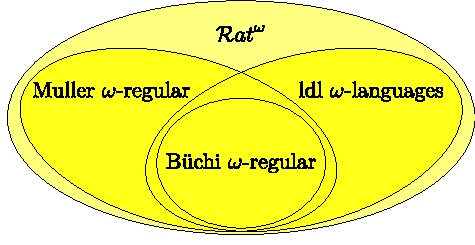
\includegraphics[width=0.95\linewidth,height=0.45\textheight,keepaspectratio]{graphic-11.pdf}\end{center}
 
Figure 10: Inclusion of classes of $\omega$-languages, with Büchi $\subsetneq$ Muller $\subsetneq{\mathcal{R}at}^{\omega}$.\par
 
% END S5.F10
 
% END S5.SS3.SSS0.P0.SPx2
 
% END S5.SS3
 
% END S5


% BEGIN S6
 
\par\medskip\noindent\textbf{6 Conclusion and future work}\par
 
% BEGIN S6.p1
 
We have defined interval $\omega$-pomsets with interfaces ($\omega$-iipomsets), shown that isomorphisms between them are unique, and that they admit a unique sparse decomposition. Then, we have introduced $\omega$-higher-dimensional automata ($\omega$-HDAs) over $\omega$-iipomsets as a generalization of HDAs over finite iipomsets. We have studied their languages under Büchi and Muller acceptance conditions and demonstrated that Muller is more expressive than Büchi.\par
 
% END S6.p1
 
% BEGIN S6.p2
 
Unlike in the finite case, languages of $\omega$-HDAs are not closed under subsumption. In pursuit of a Kleene-like theorem, we have adapted the rational operations on finite iipomsets to disregard subsumption, showing that up to subsumption, the notion of rational language remains unchanged under this modification. We have also introduced a non-nested $\omega$-iteration to these operations and defined $\omega$-rational languages over $\omega$-iipomsets. However, we show that this natural class is bigger than the one of $\omega$-iipomset languages recognized by $\omega$-HDAs. The diagram in Fig. 10 summarizes our results about $\omega$-HDAs and $\omega$-rational languages. In the diagram, the inclusion of Büchi $\omega$-regular languages into locally down-closed lasso $\omega$-languages is shown as strict (cf. Th. 39); but we conjecture it to be an equivalence.\par
 
% END S6.p2
 
% BEGIN S6.p3
 
The challenge in establishing a Kleene-like theorem arises from the precubical identities that force some factors to be subsumption-closed. A solution may be found by passing to the partial HDAs of [21, 13]. Intuitively, partial HDAs relax the face maps to be partial functions, satisfying precubical inclusions rather than precubical identities. However, while the language theory of HDAs has seen much recent progress, partial HDAs remain largely unexplored. The use of such objects is particularly relevant, as with our adapted rational operations, we have shown that the language of any ST-automaton is ($\omega$-)rational, which is not the case for the subsumption-closed rational operations of [19]. This notably implies that “our” rational languages are closed under bounded-width complement, whereas the original definition is only closed under bounded pseudocomplement [7].\par
 
% END S6.p3
 
% BEGIN S6.p4
 
This work represents a first step toward developing a theory of $\omega$-HDAs. Such a theory should be well-suited for modeling non-terminating concurrent systems with dependence and independence relations. In particular it would avoid some problems with state-space explosion; for example, an infinite execution where event $a$ must precede $b$ is modeled as the subsumption closure of the pomset with $a<b$ and all other events occurring in parallel, instead of considering all interleavings separately. Developing a logical characterization, similar to the finite case [5], would also be of interest.\par
 
% END S6.p4
  
% END S6


% BEGIN A1
 
\par\medskip\noindent\textbf{Appendix A Complementary proofs of Section 2}\par
 
% BEGIN A1.SS0.SSS0.P0.SPx1
 
\par\medskip\noindent\textbf{Proof of Proposition 3.}\par
 
% BEGIN A1.SS0.SSS0.P0.SPx1.p1
 
Let $P$ be an $\omega$-ipomset and define $P_{0}$ as the set of $<_{P}$-minimal elements of $P$ and $P_{i+1}$ the set of $<_{P}$-minimal elements of $P\setminus\{P_{0},\dots,P_{i}\}$ for all $i<\omega$. Note that each $P_{i}$ is an $<_{P}$-antichain and linearly ordered by $\dashrightarrow_{P}$. Define the binary relation $\mathcal{R}_{P}$ by $x\mathcal{R}_{P}y$ iff ($x\in P_{i}$, $y\in P_{j}$ and $i<j$) or $(x,y\in P_{i}$ and $x\dashrightarrow_{P}y$). Then $(P,\mathcal{R}_{P})$ is a strict well-order. In addition, an isomorphism between $\omega$-ipomsets $P$ and $Q$ is an isomorphism between $(P,\mathcal{R}_{P})$ and $(Q,\mathcal{R}_{Q})$. We conclude by noting that well-ordering isomorphisms are unique (see [30, Lem. 6.2]). $\hfill\blacktriangleleft$\par
 
% END A1.SS0.SSS0.P0.SPx1.p1
 
% END A1.SS0.SSS0.P0.SPx1
 
% BEGIN A1.SS0.SSS0.P0.SPx2
 
\par\medskip\noindent\textbf{Proof of Lemma 4.}\par
 
% BEGIN A1.SS0.SSS0.P0.SPx2.p1
 
Let $(P_{i})_{i\in\mathbb{N}}\in\mathsf{iPoms}^{\mathbb{N}}$ such that $S_{P_{i}}\cong T_{P_{i\text{+}1}}$, $I={\{i\in\mathbb{N}\mathrel{\big{|}}P_{i}\not\in\mathsf{Id}\}}$ is infinite and there is $m\in\mathbb{N}$ such that $\mathsf{wd}(P_{i})\leqslant m$. We want to show that it is a valid $\omega$-ipomset. It is routine to check that $P=P_{0}*P_{1}*\cdots$ is well-defined, however it can be a finite ipomset (for example for a constant sequence in $\mathsf{Id}$), or can define a not valid $\omega$-ipomset.\par
  
\par\noindent  $\blacksquare$ 
% BEGIN A1.I1.i1.p1
 
Infinity: By contradiction, suppose $P$ is finite. If so, there is an index $i_{0}$ such that, for $i>i_{0}$, $P_{i}$ does not start any event. Let $Q=P_{0}*...*P_{i_{0}}\in\mathsf{iPoms}$. For $i\in I$, $P_{i}\not\in\mathsf{Id}$ so it has to start or finish at least one event. Let $I^{\prime}=I\cap{\{i\in\mathbb{N}\mathrel{\big{|}}i>i_{0}\}}$, as $I$ is infinite, $I^{\prime}$ is infinite. For $i\in I^{\prime}$, $P_{i}$ has to end at least one event of $Q$. But $|Q|$ is finite and $I^{\prime}$ is infinite, contradiction.\par
 
% END A1.I1.i1.p1
 
 
\par\noindent  $\blacksquare$ 
% BEGIN A1.I1.i2.p1
 
Finite past: Let $z\in P$, there is $j\text{ s.t.\ }z\in P_{j}$. By definition of $<_{P}$, if $y<_{P}z$ then there is $i\leqslant j$ such that $y\in P_{i}$. So the $<_{P}$-predecessors of $z$ are in $(\bigcup_{i\leqslant j}(P_{i},i))_{/x\sim f(x)}$ which is finite.\par
 
% END A1.I1.i2.p1
 
 
\par\noindent  $\blacksquare$ 
% BEGIN A1.I1.i3.p1
 
No infinite $<_{P}$-antichain: Let $A$ be an $<_{P}$-antichain, then there is $i$ such that $A\subseteq P_{i}$. So $|A|\leqslant\mathsf{wd}(P_{i})\leqslant m$, so there is no infinite $<_{P}$-antichain.\par
 
% END A1.I1.i3.p1
 
  
Thus, $P$ is a valid $\omega$-ipomset. $\hfill\blacktriangleleft$\par
 
% END A1.SS0.SSS0.P0.SPx2.p1
 
% BEGIN A1.SS0.SSS0.P0.SPx2.p2
 
The following lemma is needed for the proof of Prop. 5 (see [38] for a proof):\par
 
% END A1.SS0.SSS0.P0.SPx2.p2
 
% BEGIN Thmtheorem41
 
\par\medskip\noindent\textbf{Lemma 41.}\par
 
% BEGIN Thmtheorem41.p1
 
Let $P\in{\mathsf{iPoms}^{\omega}}$ and $E$ be its set of maximal $<_{P}$-antichains. If $\ll$ is a linear order on $E$, then $(E,\ll)\cong(\mathbb{N},<)$.\par
 
% END Thmtheorem41.p1
 
% END Thmtheorem41
 
% END A1.SS0.SSS0.P0.SPx2
 
% BEGIN A1.SS0.SSS0.P0.SPx3
 
\par\medskip\noindent\textbf{Proof of Proposition 5.}\par
 
% BEGIN A1.SS0.SSS0.P0.SPx3.p1
 
We want to prove the equivalence between (1) $P$ is an interval $\omega$-ipomset, (2) $P$ has an interval representation and (3) the order $\ll$ on maximal antichains is linear.\par
  
\par\noindent  $\blacksquare$ 
% BEGIN A1.I2.i1.p1
 
(2) $\Rightarrow$ (1) : Let $w,x,y,z\in P$ with $w<_{P}y$ and $x<_{P}z$. By (2) we take an interval representation $b,e$, then $e(w)<b(y)$, $e(x)<b(z)$. Suppose that $w\nless_{P}z$, by (2) $e(w)\nless b(z)$, as $<$ is linear on $\mathbb{N}\cup{\{+\infty\}}$, $b(z)\leqslant e(w)$, and thus $e(x)<b(y)$ so by (2), $x<_{P}y$. Thus, $w<_{P}z$ or $x<_{P}y$.\par
 
% END A1.I2.i1.p1
 
 
\par\noindent  $\blacksquare$ 
% BEGIN A1.I2.i2.p1
 
(1) $\Rightarrow$ (3) : Let $A$ and $B$ be two different maximal antichains and suppose that $A\not\ll B$ and $B\not\ll A$. Then there is $(x,y)\in A\times B$ such that $x<y$ and $(x^{\prime},y^{\prime})\in A\times B$ such that $y^{\prime}<x^{\prime}$. By (1) we have $x<x^{\prime}$ or $y^{\prime}<y$, but $A$ and $B$ are $<$-antichains, contradiction.\par
 
% END A1.I2.i2.p1
 
 
\par\noindent  $\blacksquare$ 
% BEGIN A1.I2.i3.p1
 
(3) $\Rightarrow$ (2) : By Lem. 41, we can order the set $E$ of maximal antichains of $P$ such that $E={\{A_{0},\,A_{1},\,A_{2},\,...\}}$ and $A_{0}\ll A_{1}\ll A_{2}\ll...$. We define $b(x)=\mathsf{inf}{\{i\mathrel{\big{|}}x\in X_{i}\}}$ and $e(x)=\mathsf{sup}{\{i\mathrel{\big{|}}x\in A_{i}\}}$. By definition we have $b(x)\leqslant e(x)$. Let $x,y\in P\text{ s.t.\ }x<_{P}y$, then for all $i<j$ if $x\in A_{j}$, we have $A_{i}\ll A_{j}$ so $y\not\in A_{i}$, and $y\not\in A_{j}$ (otherwise $X_{j}$ is not an antichain), thus $e(x)<b(y)$. Let $x,y\in P\text{ s.t.\ }x\not<_{P}y$. Either $y<_{P}x$, then by the previous point $e(y)<b(x)$ and so $b(y)<e(x)$, or we have $y\not<_{P}x$ thus ${\{x,y\}}$ is include in a maximal antichain of $P$, then there is $i$ such that $x,y\in A_{i}$ and so $b(y)\leqslant i\leqslant e(x)$. Thus $x<_{P}y\Leftrightarrow e(x)<b(y)$.\par
 
% END A1.I2.i3.p1
 
  
So we have (1) $\Leftrightarrow$ (2) $\Leftrightarrow$ (3). $\hfill\blacktriangleleft$\par
 
% END A1.SS0.SSS0.P0.SPx3.p1
 
% BEGIN A1.SS0.SSS0.P0.SPx3.p2
 
Before proving Th. 7 we need lemma that characterize the nature (starter versus terminator) of the first element of the decomposition (Lem. 43), and one that characterise it solely from the $P$ considered (Lem. 44). We define $P^{m}$ the $<_{P}$-minimal elements of $P$ (which can be seen as a conclist with the induced event order of $P$) and $P^{s}:={\{p\in P\mathrel{\big{|}}\forall q\in P-P^{m},\,p<q\}}\subseteq P^{m}$.\par
 
% END A1.SS0.SSS0.P0.SPx3.p2
 
% BEGIN Thmtheorem42
 
\par\medskip\noindent\textbf{Lemma 42.}\par
 
% BEGIN Thmtheorem42.p1
 
Let $P=P_{0}*P_{1}*\dots$ be a sparse decomposition, then $P_{0}=P^{m}$ (seen as conclists).\par
 
% END Thmtheorem42.p1
 
% END Thmtheorem42
 
% END A1.SS0.SSS0.P0.SPx3
 
% BEGIN A1.SS0.SSS0.P0.SPx4
 
\par\medskip\noindent\textbf{Proof of Lemma 42.}\par
 
% BEGIN A1.SS0.SSS0.P0.SPx4.p1
 
By definition, we already have that $P_{0}\subseteq P^{m}$. Let’s show that $P-P_{0}\subseteq P-P^{m}$ (which is equivalent to $P^{m}\subseteq P_{0}$). Let $x\in P-P_{0}$, there is $i\geqslant 1\text{ s.t.\ }x\in P_{i}-S_{P_{i}}$.\par
  
\par\noindent  $\blacksquare$ 
% BEGIN A1.I3.i1.p1
 
If $P_{0}$ is a (proper) terminator: it exists $y\in P_{0}-T_{P_{0}}$ and thus $y<x$\par
 
% END A1.I3.i1.p1
 
 
\par\noindent  $\blacksquare$ 
% BEGIN A1.I3.i2.p1
 
If $P_{0}$ is a starter: then $P_{1}$ is a (proper) terminator so it exists $y\in P_{1}-T_{P_{1}}$, and $i\geqslant 2$ (because $P_{1}=S_{P_{1}}$), thus $y<x$\par
 
% END A1.I3.i2.p1
 
  
In both cases there is an element before $x$ so $x\not\in P^{m}$, so $P-P_{0}\subseteq P-P^{m}$. $\hfill\blacktriangleleft$\par
 
% END A1.SS0.SSS0.P0.SPx4.p1
 
% BEGIN Thmtheorem43
 
\par\medskip\noindent\textbf{Lemma 43.}\par
 
% BEGIN Thmtheorem43.p1
 
Let $P=P_{0}*P_{1}*\dots$ be a sparse decomposition, then $P_{0}$ is a starter iff $S_{P}\subsetneq P^{m}$ (equivalently, $P_{0}$ is a terminator iff $S_{P}=P^{m}$).\par
 
% END Thmtheorem43.p1
 
% END Thmtheorem43
 
% END A1.SS0.SSS0.P0.SPx4
 
% BEGIN A1.SS0.SSS0.P0.SPx5
 
\par\medskip\noindent\textbf{Proof of Lemma 43.}\par
 
% BEGIN A1.SS0.SSS0.P0.SPx5.p1
 
Using Lem. 42, $P_{0}=P^{m}$, and by definition $S_{P_{0}}=S_{P}$. Then we have that $P_{0}$ is a starter iff $S_{P}=S_{P_{0}}\subsetneq P_{0}=P^{m}$. $\hfill\blacktriangleleft$\par
 
% END A1.SS0.SSS0.P0.SPx5.p1
 
% BEGIN Thmtheorem44
 
\par\medskip\noindent\textbf{Lemma 44.}\par
 
% BEGIN Thmtheorem44.p1
 
Let $P=P_{0}*P_{1}*\dots$ be a sparse decomposition:\par
  
\par\noindent  $\blacksquare$ 
% BEGIN A1.I4.i1.p1
 
If $P_{0}$ is a starter, $P_{0}=\ {}_{P^{m}-S_{P}\!}{\uparrow}{P^{m}}$\par
 
% END A1.I4.i1.p1
 
 
\par\noindent  $\blacksquare$ 
% BEGIN A1.I4.i2.p1
 
If $P_{0}$ is a terminator, $P_{0}={P^{m}}{\downarrow}_{P^{s}}$\par
 
% END A1.I4.i2.p1
 
  
% END Thmtheorem44.p1
 
% END Thmtheorem44
 
% END A1.SS0.SSS0.P0.SPx5
 
% BEGIN A1.SS0.SSS0.P0.SPx6
 
\par\medskip\noindent\textbf{Proof of Lemma 44.}\par
 
% BEGIN A1.SS0.SSS0.P0.SPx6.p1
 
Using Lem. 42, $P_{0}=P^{m}$:\par
  
\par\noindent  $\blacksquare$ 
% BEGIN A1.I5.i1.p1
 
If $P_{0}$ is a starter, by Lem. 43 $S_{P}=S_{P_{0}}\subsetneq P_{0}=P^{m}$ and so $P_{0}={}_{P_{0}-S_{P_{0}}\!}{\uparrow}{P_{0}}={}_{P^{m}-S_{P}\!}{\uparrow}{P^{m}}$.\par
 
% END A1.I5.i1.p1
 
 
\par\noindent  $\blacksquare$ 
% BEGIN A1.I5.i2.p1
 
If $P_{0}$ is a terminator, we want to show that $P^{s}=P^{m}-T_{P_{0}}$, thus $P_{0}={P^{m}}{\downarrow}_{P^{s}}$. First let $p\in T_{P_{0}}$, then $p\in S_{P_{1}}\subseteq P_{1}$. $P_{1}$ is a (proper) starter so there is $q\in P_{1}-S_{P_{1}}$ so $q\not\in P_{0}=P^{m}$ and $p\not<q$ so $p\not\in P^{s}$, thus $P^{s}\subseteq P^{m}-T_{P_{0}}$. Then let $p\in P^{m}-T_{P_{0}}=P_{0}-T_{P_{0}}$ and $q\in P-P^{m}=P-P_{0}$, thus there is $i\geqslant 1\text{ s.t.\ }q\in P_{i}-S_{P_{i}}$, so $p<q$. Thus $p\in P^{s}$ and $P^{m}-T_{P_{0}}\subseteq P^{s}$.\par
 
% END A1.I5.i2.p1
 
  
Which concludes the proof. $\hfill\blacktriangleleft$\par
 
% END A1.SS0.SSS0.P0.SPx6.p1
 
% BEGIN A1.SS0.SSS0.P0.SPx6.p2
 
We can now prove the fundamental decomposition of $\omega$-iipomsets:\par
 
% END A1.SS0.SSS0.P0.SPx6.p2
 
% END A1.SS0.SSS0.P0.SPx6
 
% BEGIN A1.SS0.SSS0.P0.SPx7
 
\par\medskip\noindent\textbf{Proof of Theorem 7.}\par
 
% BEGIN A1.SS0.SSS0.P0.SPx7.p1
 
Let $P\in{\mathsf{iiPoms}^{\omega}}$, by Lem. 41, as $\ll$ is linear by Prop. 5, we have that $X_{0}\ll X_{1}\ll\dots$ . For all $i\in\mathbb{N}$, we can define $E_{i}=X_{i}-X_{i\text{+}1}$ and $B_{i}=X_{i\text{+}1}-X_{i}$. As $X_{i}$ are maximal antichains, the sets are not empty and $\forall(x,y)\in E_{i}\times B_{i},\,x<_{P}y$. We then define $U_{2i}={X_{i}}{\downarrow}_{E_{i}}$ and $U_{2i\text{+}1}=\ {}_{B_{i}\!}{\uparrow}{X_{i\text{+}1}}$ which are proper (the event order on $U_{2i}$ and $U_{2i\text{+}1}$ is the one induced by $\dashrightarrow_{P}$). If $S_{P}\subsetneq X_{0}$, we shift all indices by 1 and redefine $U_{0}={}_{X_{0}-S_{P}\!}{\uparrow}{X_{0}}$. Thus $U_{0}*U_{1}*U_{2}*\dots$ is a sparse decomposition, and it is routine to check that $P=U_{0}*U_{1}*U_{2}\dots$, concluding of the existence of a sparse decomposition.\par
 
% END A1.SS0.SSS0.P0.SPx7.p1
 
% BEGIN A1.SS0.SSS0.P0.SPx7.p2
 
Let $P=P_{0}*P_{1}*\dots=Q_{0}*Q_{1}*\dots$ be two different sparse decompositions. Without loss of generality, we can delete the common prefix and consider that $P_{0}\neq Q_{0}$. If $S_{P}\subsetneq P^{m}$, by Lem. 43 $P_{0}$ and $Q_{0}$ are (proper) starters, and by Lem. 44, $P_{0}={}_{P^{m}-S_{P}\!}{\uparrow}{P^{m}}=Q_{0}$. If $S_{P}=P^{m}$, by Lem. 43 $P_{0}$ and $Q_{0}$ are (proper) terminators, and by Lem. 44, $P_{0}={P^{m}}{\downarrow}_{P^{s}}=Q_{0}$, so contradiction. $\hfill\blacktriangleleft$\par
 
% END A1.SS0.SSS0.P0.SPx7.p2
 
% END A1.SS0.SSS0.P0.SPx7
 
% BEGIN A1.SS0.SSS0.P0.SPx8
 
\par\medskip\noindent\textbf{Proof of Propoposition 12.}\par
 
% BEGIN A1.SS0.SSS0.P0.SPx8.p1
 
We show the equivalence between (1) $P$ is an interval $\omega$-ipomset, (4) all prefixes of $P$ are interval ipomsets and $\mathsf{Pref}(P)$ is infinite, and (5) an infinite number of prefixes of $P$ are interval ipomsets.\par
  
\par\noindent  $\blacksquare$ 
% BEGIN A1.I6.i1.p1
 
(1) $\Rightarrow$ (4) : Suppose for all $w,x,y,z\in P$ where $w<y$ and $x<z$, then $w<z$ or $x<y$. Then for all $A\in\mathsf{Pref}(P)$, we have the same property for all $w,x,y,z\in A\subseteq P$. Moreover, $\mathsf{Pref}(P)$ is infinite as a direct consequence of the existence part of Th. 7.\par
 
% END A1.I6.i1.p1
 
 
\par\noindent  $\blacksquare$ 
% BEGIN A1.I6.i2.p1
 
(4) $\Rightarrow$ (5) : Trivial.\par
 
% END A1.I6.i2.p1
 
 
\par\noindent  $\blacksquare$ 
% BEGIN A1.I6.i3.p1
 
(5) $\Rightarrow$ (1) : Let $(A_{i})_{i\in I}$ be the infinite set of interval ipomsets in $\mathsf{Pref}(P)$. Let $w,x,y,z\in P$ where $w<y$, $x<z$. By Lem. 10, there is a prefix $A_{i}$ with ${\{w,x,y,z\}}\subseteq A_{i}$, which is an interval ipomset, then $w<y$ or $x<z$.\par
 
% END A1.I6.i3.p1
 
  
Which concludes the proof. $\hfill\blacktriangleleft$\par
 
% END A1.SS0.SSS0.P0.SPx8.p1
 
% END A1.SS0.SSS0.P0.SPx8
 
% END A1


% BEGIN A2
 
\par\medskip\noindent\textbf{Appendix B Complementary proofs of Section 5}\par
 
% BEGIN A2.SS0.SSS0.P0.SPx1
 
\par\medskip\noindent\textbf{Proof of Lemma 25.}\par
 
% BEGIN A2.SS0.SSS0.P0.SPx1.p1
 
Let $A=(Q,E,I,F,\lambda)$ be an ST-automaton. As $\lambda$ is coherent with $E$, all interfaces coincide in a word produced by $A$. Then it remains to show that the languages does not contain not allowed words.\par
 
% END A2.SS0.SSS0.P0.SPx1.p1
 
% BEGIN A2.SS0.SSS0.P0.SPx1.p2
 
If $A$ accepts finite words, then even for a path of one states $q$, the label contains at least the letter $\mathsf{id}_{\lambda(q)}$. Thus $\varepsilon\not\in L(A)$, and $L(A)\subseteq\mathsf{Coh}^{+}(\overline{\Xi})$.\par
 
% END A2.SS0.SSS0.P0.SPx1.p2
 
% BEGIN A2.SS0.SSS0.P0.SPx1.p3
 
If $A$ accepts infinite words, then for every infinite path, one letter out of two is in $\overline{\Xi}\setminus\mathsf{Id}$, so there is an infinite number of non-identity letters, thus $L(A)\subseteq\mathsf{Coh}^{\omega}(\overline{\Xi})$. $\hfill\blacktriangleleft$\par
 
% END A2.SS0.SSS0.P0.SPx1.p3
 
% END A2.SS0.SSS0.P0.SPx1
 
% BEGIN A2.SS0.SSS0.P0.SPx2
 
\par\medskip\noindent\textbf{Proof of Lemma 27.}\par
 
% BEGIN A2.SS0.SSS0.P0.SPx2.p1
 
Let $\alpha=(q_{0},\varphi_{0},q_{1},...)$ be an $\omega$-track in $X$ and $ST(\alpha)=(q_{0},e_{0},q_{1},...)$ with $e_{i}=(q_{i},P_{i},q_{i\text{+}1})$. By definition:\par
  
\par\noindent  $\blacksquare$ 
% BEGIN A2.I1.i1.p1
 
If $(q_{i},\varphi_{i},q_{i\text{+}1})=(\delta_{A_{i}}^{0}(q_{i\text{+}1}),\mathrel{\nearrow^{A_{i}}},q_{i\text{+}1})$, then $P_{i}=\mathsf{ev}(q_{i},\varphi_{i},q_{i\text{+}1})$\par
 
% END A2.I1.i1.p1
 
 
\par\noindent  $\blacksquare$ 
% BEGIN A2.I1.i2.p1
 
If $(q_{i},\varphi_{i},q_{i\text{+}1})=(q_{i},\mathrel{\searrow_{A_{i}}},\delta_{A_{i}}^{1}(q_{i}))$, then $P_{i}=\mathsf{ev}(q_{i},\varphi_{i},q_{i\text{+}1})$\par
 
% END A2.I1.i2.p1
 
  
We recall that $\lambda$ is coherent, so for $(q_{i},e_{i},q_{i\text{+}1})\in E$ we have $\lambda(q_{i})=T_{P_{i}}$, $\lambda(q_{i\text{+}1})=S_{P_{i\text{+}1}}$, hence:\par
 
% END A2.SS0.SSS0.P0.SPx2.p1
 
% BEGIN A2.SS0.SSS0.P0.SPx2.p2
 
\begin{center}\resizebox{\linewidth}{!}{$\begin{aligned}\displaystyle\mathsf{ev}(\alpha) & \displaystyle=\ \mathsf{ev}(q_{0},\varphi_{0},q_{1})*\mathsf{ev}(q_{1},\varphi_{1},q_{2})*\cdots=\ P_{0}*P_{1}*\cdots=\ \mathsf{id}_{\lambda(q_{0})}*P_{0}*\mathsf{id}_{\lambda(q_{1})}*P_{1}*\cdots\\\displaystyle=\ \Psi(\mathsf{id}_{\lambda(q_{0})}\cdot P_{0}\cdot\mathsf{id}_{\lambda(q_{1})}\cdot P_{1}\cdot\ldots)=\ \Psi(l(ST(\alpha)))\ \end{aligned}$}\end{center}
 
$\hfill\blacktriangleleft$\par
 
% END A2.SS0.SSS0.P0.SPx2.p2
 
% END A2.SS0.SSS0.P0.SPx2
 
% BEGIN A2.SS0.SSS0.P0.SPx3
 
\par\medskip\noindent\textbf{Proof of Lemma 29.}\par
 
% BEGIN A2.SS0.SSS0.P0.SPx3.p1
 
For an expression $e_{A}$ of finite words, we replace any occurrence of the Kleene star with the formula $L^{*}=\varepsilon+L^{+}$, and “developp” the expression. For ST-automaton $A$, $\varepsilon\not\in L(A)$, the resulting expression after developing is such that there is no $\varepsilon$ anymore.\par
 
% END A2.SS0.SSS0.P0.SPx3.p1
 
% BEGIN A2.SS0.SSS0.P0.SPx3.p2
 
For an $\omega$-rational expression $e_{A^{\prime}}$, we know that $e_{A^{\prime}}$ can be a finite union of the form $\bigcup X.Y^{\omega}$ with $X$ and $Y$ rational sets of finite words (see Th. 3.2 of [39]). It suffices to show that we can remove the occurrences of ∗ and $\varepsilon$ for an expression $X.Y^{\omega}$. We replace any occurrences of the Kleene star by $L^{*}=\varepsilon+L^{+}$. Then we develop the expression such that:\par
  
\par\noindent  $\blacksquare$ 
% BEGIN A2.I2.i1.p1
 
If $\varepsilon\in X$, $X=\varepsilon+X^{\prime}$ (with $\varepsilon\not\in X^{\prime}$) and $X.Y^{\omega}=Y^{\omega}+X^{\prime}.Y^{\omega}=Y.Y^{\omega}+X^{\prime}.Y^{\omega}$\par
 
% END A2.I2.i1.p1
 
 
\par\noindent  $\blacksquare$ 
% BEGIN A2.I2.i2.p1
 
If $\varepsilon\in Y$, $Y=\varepsilon+Y^{\prime}$ (with $\varepsilon\not\in Y^{\prime}$) and because of the definition of \ensuremath{\omega}, we have $X.Y^{\omega}=X.Y^{\prime}\ {}^{\omega}$\par
 
% END A2.I2.i2.p1
 
  
Thus we can transform $e_{A}$ into a positive expression $\overline{e}_{A}$ (resp. $e_{A^{\prime}}$ into $\overline{e}_{A^{\prime}}$). For a formula over infinite words, it is moreover still of the form $\bigcup X.Y^{\omega}$. $\hfill\blacktriangleleft$\par
 
% END A2.SS0.SSS0.P0.SPx3.p2
 
% END A2.SS0.SSS0.P0.SPx3
 
% BEGIN A2.SS0.SSS0.P0.SPx4
 
\par\medskip\noindent\textbf{Proof of Lemma 32.}\par
 
% BEGIN A2.SS0.SSS0.P0.SPx4.p1
 
Let $A$ be an ST-automaton of finite words. The ST-automaton is finite, so by the classical Kleene theorem, $L(A)$ can be represented by a rational expression $e_{A}(U_{1},...,U_{n})$, written $e_{A}$ for simplification. We have $\mathcal{L}(e_{A})=L(A)$. By Lem 29 , we can suppose $e_{A}$ to be positive, and by Lem 31, $\Psi(L(A))=\Psi(\mathcal{L}(e_{A}))=\Psi^{\prime}(e_{A})$. By Lem 30, $\Psi^{\prime}(e_{A})\in\mathcal{R}at$, so $\Psi(L(A))\in\mathcal{R}at$.\par
 
% END A2.SS0.SSS0.P0.SPx4.p1
 
% BEGIN A2.SS0.SSS0.P0.SPx4.p2
 
The same can be done for an ST-automaton of infinite words $A^{\prime}$. By the $\omega$-Kleene theorem (for example shown in [39]), $L(A^{\prime})$ can be represented by a $\omega$-rational positive expression $e_{A^{\prime}}$, with $\mathcal{L}(e_{A^{\prime}})=L(A^{\prime})$, and we have $\Psi(L(A^{\prime}))=\Psi(\mathcal{L}(e_{A^{\prime}})=\Psi^{\prime}(e_{A^{\prime}})$, and by Lem 30, $\Psi(L(A^{\prime}))\in{\mathcal{R}at}^{\omega}$. $\hfill\blacktriangleleft$\par
 
% END A2.SS0.SSS0.P0.SPx4.p2
 
% BEGIN A2.SS0.SSS0.P0.SPx4.p3
 
The following results are needed for the induction part of the proof of Prop. 36:\par
 
% END A2.SS0.SSS0.P0.SPx4.p3
 
% BEGIN Thmtheorem45
 
\par\medskip\noindent\textbf{Lemma 45.}\par
 
% BEGIN Thmtheorem45.p1
 
For $L,M\subseteq\mathsf{iiPoms}$, $(L*M)\mathord{\downarrow}=L\mathord{\downarrow}*_{\mathord{\downarrow}}M\mathord{\downarrow}$.\par
 
% END Thmtheorem45.p1
 
% END Thmtheorem45
 
% END A2.SS0.SSS0.P0.SPx4
 
% BEGIN A2.SS0.SSS0.P0.SPx5
 
\par\medskip\noindent\textbf{Proof of Lemma 45.}\par
 
% BEGIN A2.SS0.SSS0.P0.SPx5.p1
 
Let $P\in(L*M)\mathord{\downarrow}$, there is $A\in L$ and $B\in M$ such that $P\sqsubseteq A*B$. As $L\subseteq L\mathord{\downarrow}$ and $M\subseteq M\mathord{\downarrow}$, $A*B\in L\mathord{\downarrow}*M\mathord{\downarrow}$ so $P\in(L\mathord{\downarrow}*M\mathord{\downarrow})\mathord{\downarrow}=L\mathord{\downarrow}*_{\mathord{\downarrow}}M\mathord{\downarrow}$ and $(L*M)\mathord{\downarrow}\subseteq L\mathord{\downarrow}*_{\mathord{\downarrow}}M\mathord{\downarrow}$.\par
 
% END A2.SS0.SSS0.P0.SPx5.p1
 
% BEGIN A2.SS0.SSS0.P0.SPx5.p2
 
Let $Q\in L\mathord{\downarrow}*_{\mathord{\downarrow}}M\mathord{\downarrow}$, there is $A\in L\mathord{\downarrow}$ and $B\in M\mathord{\downarrow}$ such that $Q\sqsubseteq A*B$. There is $A^{\prime}\in L$ such that $A\sqsubseteq A^{\prime}$ and $B^{\prime}\in M$ such that $B\sqsubseteq B^{\prime}$. By Lem. 48 of [18], $A*B\sqsubseteq A^{\prime}*B^{\prime}$ and by transitivity, $Q\sqsubseteq A^{\prime}*B^{\prime}$. But we have $A^{\prime}*B^{\prime}\in L*M$, so $Q\in(L*M)\mathord{\downarrow}$ and $L\mathord{\downarrow}*_{\mathord{\downarrow}}M\mathord{\downarrow}\subseteq(L*M)\mathord{\downarrow}$. $\hfill\blacktriangleleft$\par
 
% END A2.SS0.SSS0.P0.SPx5.p2
 
% BEGIN Thmtheorem46
 
\par\medskip\noindent\textbf{Corollary 46.}\par
 
% BEGIN Thmtheorem46.p1
 
For $L,M\subseteq\mathsf{iiPoms}$, $(L^{+})\mathord{\downarrow}=(L\mathord{\downarrow})^{+_{\mathord{\downarrow}}}$.\par
 
% END Thmtheorem46.p1
 
% END Thmtheorem46
 
% END A2.SS0.SSS0.P0.SPx5
 
% BEGIN A2.SS0.SSS0.P0.SPx6
 
\par\medskip\noindent\textbf{Proof of Proposition 36.}\par
 
% BEGIN A2.SS0.SSS0.P0.SPx6.p1
 
We start by showing that $\mathcal{R}at\mathord{\downarrow}\subseteq D\text{-}\mathcal{R}at$ by induction:\par
  
\par\noindent  $\blacksquare$ 
% BEGIN A2.I3.i1.p1
 
$\emptyset\mathord{\downarrow}=\emptyset\in D\text{-}\mathcal{R}at$\par
 
% END A2.I3.i1.p1
 
 
\par\noindent  $\blacksquare$ 
% BEGIN A2.I3.i2.p1
 
For $U\in\Xi$, ${\{U\}}\mathord{\downarrow}={\{U\}}$ (as $<_{U}$ is empty) and ${\{U\}}\in D\text{-}\mathcal{R}at$ (by a finite use of $\parallel_{\mathord{\downarrow}}$ and ${\{a\vbox{\hbox{\tiny$\bullet$}}\}}$ and ${\{\vbox{\hbox{\tiny$\bullet$}}a\vbox{\hbox{\tiny$\bullet$}}\}}$, or ${\{\vbox{\hbox{\tiny$\bullet$}}a\}}$ and ${\{\vbox{\hbox{\tiny$\bullet$}}a\vbox{\hbox{\tiny$\bullet$}}\}}$, for $a\in\Sigma$)\par
 
% END A2.I3.i2.p1
 
 
\par\noindent  $\blacksquare$ 
% BEGIN A2.I3.i3.p1
 
For $L,M\in\mathcal{R}at$, if $L\mathord{\downarrow},M\mathord{\downarrow}\in D\text{-}\mathcal{R}at$, then $(L+M)\mathord{\downarrow}=L\mathord{\downarrow}+M\mathord{\downarrow}\in D\text{-}\mathcal{R}at$\par
 
% END A2.I3.i3.p1
 
 
\par\noindent  $\blacksquare$ 
% BEGIN A2.I3.i4.p1
 
For $L,M\in\mathcal{R}at$, if $L\mathord{\downarrow},M\mathord{\downarrow}\in D\text{-}\mathcal{R}at$, then $(L*M)\mathord{\downarrow}=L\mathord{\downarrow}*_{\mathord{\downarrow}}M\mathord{\downarrow}\in D\text{-}\mathcal{R}at$ (by Lem. 45)\par
 
% END A2.I3.i4.p1
 
 
\par\noindent  $\blacksquare$ 
% BEGIN A2.I3.i5.p1
 
For $L\in\mathcal{R}at$, if $L\mathord{\downarrow}\in D\text{-}\mathcal{R}at$, then $(L^{+})\mathord{\downarrow}=(L\mathord{\downarrow})^{+_{\mathord{\downarrow}}}\in D\text{-}\mathcal{R}at$ (by Cor. 46)\par
 
% END A2.I3.i5.p1
 
  
Then by induction $\mathcal{R}at\mathord{\downarrow}\subseteq D\text{-}\mathcal{R}at$.\par
 
% END A2.SS0.SSS0.P0.SPx6.p1
 
% BEGIN A2.SS0.SSS0.P0.SPx6.p2
 
Next we show that $D\text{-}\mathcal{R}at\subseteq\mathcal{R}at$, which is just a more detailed version of the Remark 7.3 of [19]. Let $L\in D\text{-}\mathcal{R}at$, by Th. 17 there is a HDA $X$ such that $L=L(X)$. Let $ST(X)$ be its ST-automata, by Prop. 26 $L(X)=\Psi(L(ST(X)))$, and by Lem. 32, $\Psi(L(ST(X)))\in\mathcal{R}at$. Thus $D\text{-}\mathcal{R}at\subseteq\mathcal{R}at$.\par
 
% END A2.SS0.SSS0.P0.SPx6.p2
 
% BEGIN A2.SS0.SSS0.P0.SPx6.p3
 
But $L\in D\text{-}\mathcal{R}at$, $L$ is down-closed (by Prop. 16 and Th. 17) so as $L\in\mathcal{R}at$, $L=L\mathord{\downarrow}\in\mathcal{R}at\mathord{\downarrow}$. Then $D\text{-}\mathcal{R}at\subseteq\mathcal{R}at\mathord{\downarrow}$. $\hfill\blacktriangleleft$\par
 
% END A2.SS0.SSS0.P0.SPx6.p3
 
% END A2.SS0.SSS0.P0.SPx6
 
% BEGIN A2.SS0.SSS0.P0.SPx7
 
\par\medskip\noindent\textbf{Proof of Theorem 39.}\par
 
% BEGIN A2.SS0.SSS0.P0.SPx7.p1
 
We use the key property that language of a classical Büchi automaton $A=(Q,E,I,F)$ is of the form $\bigcup_{q_{i}\in I,\,q_{f}\in F}W(q_{i},q_{f}).W(q_{f},q_{f})^{\omega}$, where $W(p,q)$ is the language of the Büchi automaton $(Q,E,{\{p\}},{\{q\}})$ (see [24] for more details).\par
 
% END A2.SS0.SSS0.P0.SPx7.p1
 
% BEGIN A2.SS0.SSS0.P0.SPx7.p2
 
Let $(X,\bot_{X},\top_{X})$ be a Büchi $\omega$-HDA, and $ST(X)=(Q,E,I,F,\lambda)$ be its ST-automaton. Thus $L(ST(X))=\mathcal{L}(\bigcup_{q_{i}\in I,\,q_{f}\in F}W(q_{i},q_{f}).W(q_{f},q_{f})^{\omega})$. To simplify, we write $W_{1}=W(q_{i},q_{f})$ and $W_{2}=W(q_{f},q_{f})$. As, $W_{2}=(W_{2})^{+}+\varepsilon$ so we have $L(ST(X))=\mathcal{L}(\bigcup W_{1}.((W_{2})^{+})^{\omega})$.\par
 
% END A2.SS0.SSS0.P0.SPx7.p2
 
% BEGIN A2.SS0.SSS0.P0.SPx7.p3
 
But $\mathcal{L}(W_{1})$ and $\mathcal{L}(W_{2})$ are languages of ST-automata from HDAs (over finite tracks), so by Prop. 36 it exists $X,Y\subseteq\mathsf{iiPoms}$ such that $\Psi(\mathcal{L}(W_{1}))=X\mathord{\downarrow}$ and $\Psi(\mathcal{L}(W_{2}))=Y\mathord{\downarrow}$. Then:\par
 
\begin{center}\resizebox{\linewidth}{!}{$\begin{aligned}\displaystyle L(X)= & \displaystyle\ \Psi(L(ST(X)))=\ \Psi(\mathcal{L}(\bigcup W_{1}.((W_{2})^{+})^{\omega}))\\\displaystyle= & \displaystyle\ \Psi^{\prime}(\bigcup W_{1}.((W_{2})^{+})^{\omega})=\ \bigcup\Psi^{\prime}(W_{1})*(\Psi^{\prime}(W_{2})^{+})^{\omega}\\\displaystyle= & \displaystyle\ \bigcup\Psi(\mathcal{L}(W_{1}))*(\Psi(\mathcal{L}(W_{2}))^{+})^{\omega}\\\displaystyle= & \displaystyle\ \bigcup X\mathord{\downarrow}*((Y\mathord{\downarrow})^{+})^{\omega}\end{aligned}$}\end{center}
 
Which concludes the proof. $\hfill\blacktriangleleft$\par
 
% END A2.SS0.SSS0.P0.SPx7.p3
 
% BEGIN A2.SS0.SSS0.P0.SPx7.p4
 
\par
 
% END A2.SS0.SSS0.P0.SPx7.p4
 
% END A2.SS0.SSS0.P0.SPx7
 
% END A2

\begin{thebibliography}{99}
\bibitem{bib-bib1} 
\par\noindent    Rajeev Alur, Caleb Stanford, and Christopher Watson.  A robust theory of series parallel graphs.  Proc. ACM Program. Lang., 7(POPL):1058–1088, 2023.  doi:10.1145/3571230.  

\bibitem{bib-bib2} 
\par\noindent    Amazigh Amrane, Hugo Bazille, Emily Clement, and Uli Fahrenberg.  Languages of higher-dimensional timed automata.  In Lars Michael Kristensen and Jan Martijn E. M. van der Werf, editors, Application and Theory of Petri Nets and Concurrency - 45th International Conference, PETRI NETS 2024, Geneva, Switzerland, June 26-28, 2024, Proceedings, volume 14628 of Lecture Notes in Computer Science, pages 197–219. Springer, 2024.  doi:10.1007/978-3-031-61433-0\_10.  

\bibitem{bib-bib3} 
\par\noindent    Amazigh Amrane, Hugo Bazille, Emily Clement, Uli Fahrenberg, and Philipp Schlehuber-Caissier.  Higher-dimensional timed automata for real-time concurrency.  In Andreas Rauh, Bernd Finkbeiner, and Paul Kröger, editors, Design and Verification of Cyber-Physical Systems. Springer, 2025.  To be published. https://arxiv.org/abs/2401.17444.  

\bibitem{bib-bib4} 
\par\noindent    Amazigh Amrane, Hugo Bazille, Emily Clement, Uli Fahrenberg, and Krzysztof Ziemianski.  Presenting interval pomsets with interfaces.  In Uli Fahrenberg, Wesley Fussner, and Roland Glück, editors, Relational and Algebraic Methods in Computer Science - 21st International Conference, RAMiCS 2024, Prague, Czech Republic, August 19-22, 2024, Proceedings, volume 14787 of Lecture Notes in Computer Science, pages 28–45. Springer, 2024.  doi:10.1007/978-3-031-68279-7\_3.  

\bibitem{bib-bib5} 
\par\noindent    Amazigh Amrane, Hugo Bazille, Uli Fahrenberg, and Marie Fortin.  Logic and languages of higher-dimensional automata.  In International Conference on Developments in Language Theory, pages 51–67. Springer, 2024.  doi:10.1007/978-3-031-66159-4\_5.  

\bibitem{bib-bib6} 
\par\noindent    Amazigh Amrane, Hugo Bazille, Uli Fahrenberg, Loïc Hélouët, and Philipp Schlehuber-Caissier.  Petri nets and higher-dimensional automata, 2025.  Accepted for PETRI NETS.  doi:10.48550/arXiv.2502.02354.  

\bibitem{bib-bib7} 
\par\noindent    Amazigh Amrane, Hugo Bazille, Uli Fahrenberg, and Krzysztof Ziemiański.  Closure and decision properties for higher-dimensional automata.  In Erika Ábrahám, Clemens Dubslaff, and Silvia Lizeth Tapia Tarifa, editors, ICTAC, volume 14446 of Lecture Notes in Computer Science, pages 295–312. Springer, 2023.  doi:10.1007/978-3-031-47963-2\_18.  

\bibitem{bib-bib8} 
\par\noindent    Amazigh Amrane, Hugo Bazille, Uli Fahrenberg, and Krzysztof Ziemiański.  Closure and decision properties for higher-dimensional automata.  Theoretical Computer Science, 1036:115156, 2025.  doi:10.1016/j.tcs.2025.115156.  

\bibitem{bib-bib9} 
\par\noindent    Marek A. Bednarczyk.  Categories of Asynchronous Systems.  PhD thesis, University of Sussex, UK, 1987.  

\bibitem{bib-bib10} 
\par\noindent    J Richard Büchi.  Symposium on decision problems: On a decision method in restricted second order arithmetic.  In Studies in Logic and the Foundations of Mathematics, volume 44, pages 1–11. Elsevier, 1966.  

\bibitem{bib-bib11} 
\par\noindent    Olivier Carton, Dominique Perrin, and Jean-Eric Pin.  Automata and semigroups recognizing infinite words.  Logic and automata, 2:133–168, 2008.  

\bibitem{bib-bib12} 
\par\noindent    Volker Diekert and Anca Muscholl.  Deterministic asynchronous automata for infinite traces.  In Annual Symposium on Theoretical Aspects of Computer Science, pages 617–628. Springer, 1993.  doi:10.1007/3-540-56503-5\_61.  

\bibitem{bib-bib13} 
\par\noindent    Jérémy Dubut.  Trees in partial higher dimensional automata.  In Mikołaj Bojańczyk and Alex Simpson, editors, FOSSACS, volume 11425 of Lecture Notes in Computer Science, pages 224–241. Springer, 2019.  doi:10.1007/978-3-030-17127-8\_13.  

\bibitem{bib-bib14} 
\par\noindent    Alexandre Duret-Lutz, Etienne Renault, Maximilien Colange, Florian Renkin, Alexandre Gbaguidi Aisse, Philipp Schlehuber-Caissier, Thomas Medioni, Antoine Martin, Jérôme Dubois, Clément Gillard, and Henrich Lauko.  From Spot 2.0 to Spot 2.10: What’s new?  In 34th International Conference on Computer Aided Verification (CAV’22), volume 13372 of Lecture Notes in Computer Science, pages 174–187. Springer, 2022.  doi:10.1007/978-3-031-13188-2\_9.  

\bibitem{bib-bib15} 
\par\noindent    Werner Ebinger and Anca Muscholl.  Logical definability on infinite traces.  Theoretical Computer Science, 154(1):67–84, 1996.  doi:10.1016/0304-3975(95)00130-1.  

\bibitem{bib-bib16} 
\par\noindent    Uli Fahrenberg.  Higher-dimensional timed automata.  In Alessandro Abate, Antoine Girard, and Maurice Heemels, editors, ADHS, volume 51 of IFAC-PapersOnLine, pages 109–114. Elsevier, 2018.  doi:10.1016/j.ifacol.2018.08.019.  

\bibitem{bib-bib17} 
\par\noindent    Uli Fahrenberg.  Higher-dimensional timed and hybrid automata.  Leibniz Transactions on Embedded Systems, 8(2):03:1–03:16, 2022.  doi:10.4230/LITES.8.2.3.  

\bibitem{bib-bib18} 
\par\noindent    Uli Fahrenberg, Christian Johansen, Georg Struth, and Krzysztof Ziemiański.  Languages of higher-dimensional automata.  Mathematical Structures in Computer Science, 31(5):575–613, 2021.  doi:10.1017/S0960129521000293.  

\bibitem{bib-bib19} 
\par\noindent    Uli Fahrenberg, Christian Johansen, Georg Struth, and Krzysztof Ziemiański.  A Kleene theorem for higher-dimensional automata.  In Bartek Klin, Sławomir Lasota, and Anca Muscholl, editors, CONCUR, volume 243 of Leibniz International Proceedings in Informatics, pages 29:1–29:18. Schloss Dagstuhl – Leibniz-Zentrum für Informatik, 2022.  doi:10.4230/LIPIcs.CONCUR.2022.29.  

\bibitem{bib-bib20} 
\par\noindent    Uli Fahrenberg, Christian Johansen, Georg Struth, and Krzysztof Ziemiański.  Posets with interfaces as a model for concurrency.  Information and Computation, 285(B):104914, 2022.  doi:10.1016/j.ic.2022.104914.  

\bibitem{bib-bib21} 
\par\noindent    Uli Fahrenberg and Axel Legay.  Partial higher-dimensional automata.  In Lawrence S. Moss and Pawel Sobocinski, editors, CALCO, volume 35 of LIPIcs, pages 101–115. Schloss Dagstuhl – Leibniz-Zentrum für Informatik, 2015.  doi:10.4230/LIPIcs.CALCO.2015.101.  

\bibitem{bib-bib22} 
\par\noindent    Uli Fahrenberg and Krzysztof Ziemiański.  A Myhill-Nerode theorem for higher-dimensional automata.  In Luís Gomes and Robert Lorenz, editors, PETRI NETS, volume 13929 of Lecture Notes in Computer Science, pages 167–188. Springer, 2023.  doi:10.1007/978-3-031-33620-1\_9.  

\bibitem{bib-bib23} 
\par\noindent    Jean Fanchon and Rémi Morin.  Pomset languages of finite step transition systems.  In Giuliana Franceschinis and Karsten Wolf, editors, PETRI NETS, volume 5606 of Lecture Notes in Computer Science, pages 83–102. Springer, 2009.  doi:10.1007/978-3-642-02424-5\_7.  

\bibitem{bib-bib24} 
\par\noindent    Berndt Farwer.  omega-automata.  In Erich Grädel, Wolfgang Thomas, and Thomas Wilke, editors, Automata, Logics, and Infinite Games: A Guide to Current Research [outcome of a Dagstuhl seminar, February 2001], volume 2500 of Lecture Notes in Computer Science, pages 3–20. Springer, 2001.  doi:10.1007/3-540-36387-4\_1.  

\bibitem{bib-bib25} 
\par\noindent    Peter C. Fishburn.  Intransitive indifference with unequal indifference intervals.  Journal of Mathematical Psychology, 7(1):144–149, 1970.  doi:10.1016/0022-2496(70)90062-3.  

\bibitem{bib-bib26} 
\par\noindent    Paul Gastin, Antoine Petit, and Wiesław Zielonka.  An extension of Kleene’s and Ochmański’s theorems to infinite traces.  Theoretical Computer Science, 125(2):167–204, 1994.  doi:10.1016/0304-3975(94)90254-2.  

\bibitem{bib-bib27} 
\par\noindent    Blaise Genest, Dietrich Kuske, and Anca Muscholl.  A Kleene theorem and model checking algorithms for existentially bounded communicating automata.  Information and Computation, 204(6):920–956, 2006.  doi:10.1016/j.ic.2006.01.005.  

\bibitem{bib-bib28} 
\par\noindent    Jay L Gischer.  The equational theory of pomsets.  Theoretical Computer Science, 61(2-3):199–224, 1988.  doi:10.1016/0304-3975(88)90124-7.  

\bibitem{bib-bib29} 
\par\noindent    Jan Grabowski.  On partial languages.  Fundamentae Informatica, 4(2):427, 1981.  

\bibitem{bib-bib30} 
\par\noindent    Kenneth Kunen.  Set Theory: An Introduction to Independence Proofs.  North-Holland, 1980.  

\bibitem{bib-bib31} 
\par\noindent    Dietrich Kuske.  Infinite series-parallel posets: Logic and languages.  In Ugo Montanari, José D. P. Rolim, and Emo Welzl, editors, Automata, Languages and Programming, 27th International Colloquium, ICALP 2000, Geneva, Switzerland, July 9-15, 2000, Proceedings, volume 1853 of Lecture Notes in Computer Science, pages 648–662. Springer, 2000.  doi:10.1007/3-540-45022-X\_55.  

\bibitem{bib-bib32} 
\par\noindent    K. Lodaya and P. Weil.  A Kleene iteration for parallelism.  In Foundations of Software Technology and Theoretical Computer Science, pages 355–366, 1998.  

\bibitem{bib-bib33} 
\par\noindent    K. Lodaya and P. Weil.  Series-parallel posets: algebra, automata and languages.  In STACS’98, volume 1373 of Lecture Notes in Computer Science, pages 555–565. Springer, 1998.  doi:10.1007/BFB0028590.  

\bibitem{bib-bib34} 
\par\noindent    K. Lodaya and P. Weil.  Series-parallel languages and the bounded-width property.  Theoretical Computer Science, 237(1–2):347–380, 2000.  doi:10.1016/S0304-3975(00)00031-1.  

\bibitem{bib-bib35} 
\par\noindent    K. Lodaya and P. Weil.  Rationality in algebras with a series operation.  Information and Computation, 171:269–293, 2001.  doi:10.1006/INCO.2001.3077.  

\bibitem{bib-bib36} 
\par\noindent    Robert McNaughton.  Testing and generating infinite sequences by a finite automaton.  Information and control, 9(5):521–530, 1966.  doi:10.1016/S0019-9958(66)80013-X.  

\bibitem{bib-bib37} 
\par\noindent    David E Muller.  Infinite sequences and finite machines.  In Proceedings of the Fourth Annual Symposium on Switching Circuit Theory and Logical Design (swct 1963), pages 3–16. IEEE Computer Society, 1963.  doi:10.1109/SWCT.1963.8.  

\bibitem{bib-bib38} 
\par\noindent    Luc Passemard, Amazigh Amrane, and Uli Fahrenberg.  Higher-dimensional automata : Extension to infinite tracks.  CoRR, abs/2503.07881, 2025.  doi:10.48550/arXiv.2503.07881.  

\bibitem{bib-bib39} 
\par\noindent    Dominique Perrin and Jean-Eric Pin.  Infinite words - automata, semigroups, logic and games, volume 141 of Pure and applied mathematics series.  Elsevier Morgan Kaufmann, 2004.  

\bibitem{bib-bib40} 
\par\noindent    Vaughan R. Pratt.  Modeling concurrency with partial orders.  Journal of Parallel Programming, 15(1):33–71, 1986.  doi:10.1007/BF01379149.  

\bibitem{bib-bib41} 
\par\noindent    Vaughan R. Pratt.  Modeling concurrency with geometry.  In POPL, pages 311–322, New York City, 1991. ACM Press.  doi:10.1145/99583.99625.  

\bibitem{bib-bib42} 
\par\noindent    Rob J. van Glabbeek.  Bisimulations for higher dimensional automata.  Email message, June 1991.  URL: http://theory.stanford.edu/˜rvg/hda.  

\bibitem{bib-bib43} 
\par\noindent    Rob J. van Glabbeek.  On the expressiveness of higher dimensional automata.  Theoretical Computer Science, 356(3):265–290, 2006.  doi:10.1016/j.tcs.2006.02.012.  

\bibitem{bib-bib44} 
\par\noindent    Glynn Winskel.  Event structures.  In W. Brauer, W. Reisig, and G. Rozenberg, editors, Petri Nets: Applications and Relationships to Other Models of Concurrency, pages 325–392, Berlin, Heidelberg, 1987. Springer Berlin Heidelberg.  

\bibitem{bib-bib45} 
\par\noindent    Glynn Winskel and Mogens Nielsen.  Models for concurrency.  In Samson Abramsky, Dov M. Gabbay, and Thomas S.E. Maibaum, editors, Handbook of Logic in Computer Science, volume 4. Clarendon Press, Oxford, 1995.  

\bibitem{bib-bib46} 
\par\noindent    Wiesław Zielonka.  Notes on finite asynchronous automata.  RAIRO – Informatique Théorique et Applications, 21(2):99–135, 1987.  doi:10.1051/ita/1987210200991.  

\end{thebibliography}
\end{document}
